En este capítulo se presentan los experimentos diseñados para evaluar la efectividad de las técnicas de selección de características y de balanceo de clases propuestas. Primero se recuerdan las preguntas de investigación del estudio empírico. Segundo, se describen los seis esquemas de selección de características, el clasificador utilizado y el flujo de trabajo. Tercero, se establece la línea base con el conjunto de datos BugHunter y el clasificador Random Forest. Luego se responden las cinco preguntas de investigación y, finalmente, se presentan tres análisis complementarios: la validación cruzada de las dos herramientas empleadas, el análisis de sensibilidad con clasificadores adicionales y un piloto exploratorio con modelos de lenguaje de gran escala.

\section{Preguntas de investigación}

El estudio empírico se realiza en dos pasos: el primero es la selección de características, para eliminar las características no relevantes y redundantes; el segundo evalúa si ese paso mejora el rendimiento de los clasificadores en la predicción final. Las cinco preguntas de investigación son:

\begin{itemize}
    \item \textbf{RQ1.} ¿El análisis de relevancia y el control de redundancia de características mejoran la identificación de errores basada en métricas de código?
    \item \textbf{RQ2.} ¿Qué métricas de código son mejores predictoras de errores y en qué nivel de granularidad (archivo, clase, método) ofrecen mejores resultados?
    \item \textbf{RQ3.} ¿Cómo influye la variación de los parámetros de los algoritmos de relevancia y redundancia en los resultados de clasificación?
    \item \textbf{RQ4.} ¿Cómo influyen los algoritmos de balanceo de clases ROS, RUS y SMOTE en los resultados de los clasificadores?
    \item \textbf{RQ5.} ¿Qué diferencias existen entre entrenar con el conjunto unificado de proyectos (proyecto resumen) y entrenar con cada proyecto por separado?
\end{itemize}

\section{Diseño experimental}
\label{sec:diseno}
En la fase de selección de características, utilizamos seis esquemas de preprocesamiento distintos. Estos esquemas se basan en la combinación de medidas de relevancia y similitud, implementadas dentro del marco propuesto por \cite{liu_empirical_2015}. Cada esquema de preprocesamiento se integra con el modelo de clasificación de RF para evaluar su eficacia utilizando el conjunto de datos BugHunter.

\subsubsection{Esquemas de Preprocesamiento}

Los seis esquemas diseñados se detallan a continuación:

\begin{enumerate}
    \item \textbf{IG + SU:} Se utiliza para el análisis de relevancia el algoritmo Ganancia de información y luego con las características resultantes se continua con el control de redundancia utilizando Incertidumbre simétrica.
    \item \textbf{CS + SU:} Se utiliza para el análisis de relevancia el algoritmo Chi-Cuadrado  y luego con las características resultantes se continua con el control de redundancia utilizando Incertidumbre simétrica.
    \item \textbf{RF + SU:} Se utiliza para el análisis de relevancia el algoritmo ReliefF y luego con las características resultantes se continua con el control de redundancia utilizando Incertidumbre simétrica.
    \item \textbf{IG + COS:} Se utiliza para el análisis de relevancia el algoritmo Ganancia de información y luego con las características resultantes se continua con el control de redundancia utilizando Semejanza de coseno.
    \item \textbf{CS + COS:} Se utiliza para el análisis de relevancia el algoritmo Chi-Cuadrado y luego con las características resultantes se continua con el control de redundancia utilizando Semejanza de coseno.
    \item \textbf{RF + COS:} Se utiliza para el análisis de relevancia el algoritmo ReliefF y luego con las características resultantes se continua con el control de redundancia utilizando Semejanza de coseno.
\end{enumerate}

Cada esquema se aplica al modelo de clasificación RF para demostrar su impacto en la eficacia de la selección de características en diferentes conjuntos de datos.

\subsubsection{Evaluación de Esquemas en el Modelo RF}

La evaluación de los esquemas se lleva a cabo mediante la integración con el modelo de clasificación RF. El objetivo es observar el rendimiento de cada esquema en términos de precision, recall y F-Measure al procesar los conjuntos de datos de BugHunter. Estos resultados ayudarán a determinar la efectividad de las combinaciones de medidas de relevancia y similitud en la etapa de selección de características.

\subsubsection{Descripción del flujo}
La figura \ref{fig:Flow} se divide en dos pasos: el \textbf{Paso 1}, de selección de características (\textit{Step 1: Features Selection} en la figura), y el \textbf{Paso 2}, de modelos de clasificación (\textit{Step 2: Classification Models}). El \textbf{Step 1} realiza la selección de características combinando análisis de relevancia (IG, CS y RF) y control de redundancia (SU, COS), teniendo como resultado un filtro del las características en los conjuntos de datos ingresados. El \textbf{Step 2} inicia dividiendo el conjunto de datos resultante del \textbf{Step 1} en entrenamiento y prueba, se mantiene un conjunto de entrenamiento original mientras se crea una copia pero balanceo el atributo clase utilizando diferentes técnicas (ROS,RUS y SMOTE) y luego se ingresan al algoritmo de clasificación quedando guardados los resultados de cada algoritmo en base de datos. 

La clasificación de características se usa para implementar el análisis de relevancia, mientras que \textbf{NTC} se usa para implementar el control de redundancia. Para la selección de características, se combina el análisis de relevancia y el control de redundancia en búsqueda de reducir la cantidad de características sin afectar los resultados de los clasificadores  \cite{liu_empirical_2015}.

El flujo descrito en la Figura \ref{fig:Flow} se realiza en diferentes iteraciones, donde el \textbf{Step 1} se itera por \(proyecto \rightarrow nivel \rightarrow k \rightarrow \beta\), teniendo como resultado las métricas seleccionadas. El \textbf{Step 2} itera \(proyecto \rightarrow nivel \rightarrow k \rightarrow \beta \rightarrow modelosSeleccion \), donde el último nivel hace referencia a los esquemas utilizados para la selección de características del \textbf{Step 1}. Esto permite que el \textbf{Step 2} ejecute los algoritmos de clasificación solo con las métricas que se seleccionaron y almacene en la base de datos los resultados.

Siendo $k$ en el proceso de \textbf{análisis de relevancia} (\textit{relevance analysis}) el valor utilizado como ranking para seleccionar las características en dependencia del orden resultante de los algoritmos  \textbf{IG, CS y RF}. En el proceso siguiente, de \textbf{control de redundancia} (\textit{redundancy check}), \(\beta \) representa el umbral para discriminar cuales métricas quedaran seleccionadas por el algoritmo \textbf {NTC}. 
Ambos pasos son explicados en detalle en los algoritmos \ref{alg:featureSelection} y \ref{alg:executionmodels}.
\begin{enumerate}
\item Selección de características (\textit{Features Selection}):
\begin{enumerate}
\item \textbf{BugHunter:} conjunto de datos almacenado en archivos CSV estructurados con la jerarquía proyecto-nivel (método, clase y archivo). Por tanto, hay 15 proyectos y 3 archivos por proyecto, un total de 45 archivos, cada uno con las métricas respectivas a su nivel. Se incluye un repositorio adicional etiquetado como \textbf{ALL} que es la unión de los 15 proyectos por cada nivel.
\item \textbf{Discretización de la clase:} proceso en el que la variable de clase se transforma en categorías. La clase original del conjunto de datos contiene un valor numerico indicando la cantidad de errores encontrados en cada registro, al ser discretizado quedan solo dos clases sin errores o con errores.
\item \textbf{Análisis de relevancia:}  para este proceso se utilizan los algoritmos IG, CS y RF, los resultados de estos algoritmos para cada característica se filtran seleccionando las k características que superen los ranking 50\%, 70\% y 90\%.
\item \textbf{Control de redundancia:} se utiliza el algoritmo NTC con los métodos SU y COS. El algoritmo es aplicado a las características seleccionadas en el paso anterior ingresando un umbral \(\beta\) (0.5, 0.7 y 0.9) el cual se encuentra en un rango entre 0 y 1. Se seleccionan aquellas características que superen el umbral ingresado a NTC.
\end{enumerate}

\item Modelos de clasificación (\textit{Classification Models}):
\begin{enumerate}
\item \textbf{División del Conjunto de Datos:} en esta fase, se procede a dividir el conjunto de datos, el cual ya incluye las métricas filtradas, en dos segmentos distintos: un \(33\%\) para el conjunto de pruebas y el \(67\%\) restante para el conjunto de entrenamiento. Para ello, se emplea la función \texttt{train\_test\_split} de la biblioteca \textit{scikit-learn} en Python. Se especifica el parámetro \texttt{stratify} con el fin de garantizar que las proporciones de las clases en los conjuntos de entrenamiento y pruebas sean representativas de las proporciones observadas en el conjunto de datos completo. Esta estrategia es crucial para mantener la consistencia y la validez estadística del proceso de validación del modelo.

\item \textbf{Balanceo de clases:} se aplican los algoritmos RUS, ROS y SMOTE para balancear la cantidad de registros con respecto a la clase. A modo de evitar que la etapa de pruebas se vea afectada por datos generados artificialmente solo se realiza el balanceo del conjunto de entrenamiento.
\item \textbf{Ejecución del modelo de clasificación:} para analizar la capacidad de los datos de predecir errores, se emplea el algoritmo de Random Forest (RF), descrito en la Sección \ref{sub:modelos}. Los conjuntos de entrenamiento y prueba generados en Python se exportan a archivos y el clasificador se ejecuta en Weka, en la modalidad \textit{Supplied test set}. Se ejecuta en dos instancias distintas para cada conjunto de datos que completa la etapa de selección de características: la primera utiliza un conjunto de entrenamiento balanceado y la segunda un conjunto sin balancear. Ambas ejecuciones comparten el mismo conjunto de pruebas para garantizar una comparación justa y coherente de los resultados.

\end{enumerate}
\end{enumerate}

\subsubsection{Orden de las etapas respecto de la partición entrenamiento/prueba}

El análisis de relevancia y el control de redundancia se calculan sobre el conjunto proyecto-nivel completo, es decir, antes de la partición en entrenamiento y prueba; el balanceo de clases, en cambio, se aplica exclusivamente dentro del conjunto de entrenamiento resultante. Dado que los tres algoritmos de relevancia (IG, CS y ReliefF) utilizan la etiqueta de clase de cada instancia, este orden introduce un riesgo de sesgo de selección: el subconjunto de características elegido puede estar influido por patrones presentes en instancias que después integrarán el conjunto de prueba \cite{ambroise2002,cawley2010}. Este riesgo afecta únicamente a la elección de qué columnas se conservan, y no a los parámetros del clasificador, que se ajustan solo con el conjunto de entrenamiento. Su magnitud se discute en el Capítulo \ref{cap:discusion}, y su corrección mediante un esquema de selección anidado se declara como trabajo futuro (Capítulo \ref{cap:conclusion}).

\subsubsection{Análisis de sensibilidad}

Para evaluar si los hallazgos dependen del clasificador, el flujo completo se repitió con \textit{Random Forest}, XGBoost y una SVM lineal, implementados en \textit{scikit-learn}, sobre la misma partición estratificada 67/33 con semilla fija y con los mismos subconjuntos de métricas. En este análisis se almacenan, además de las métricas agregadas, el \textit{F-measure} de la clase \textit{bug}, el MCC y el AUC-ROC de cada ejecución. Su diseño y resultados se presentan en la Sección \ref{sec:sensibilidad}.

\begin{figure}[H]
    \centering
    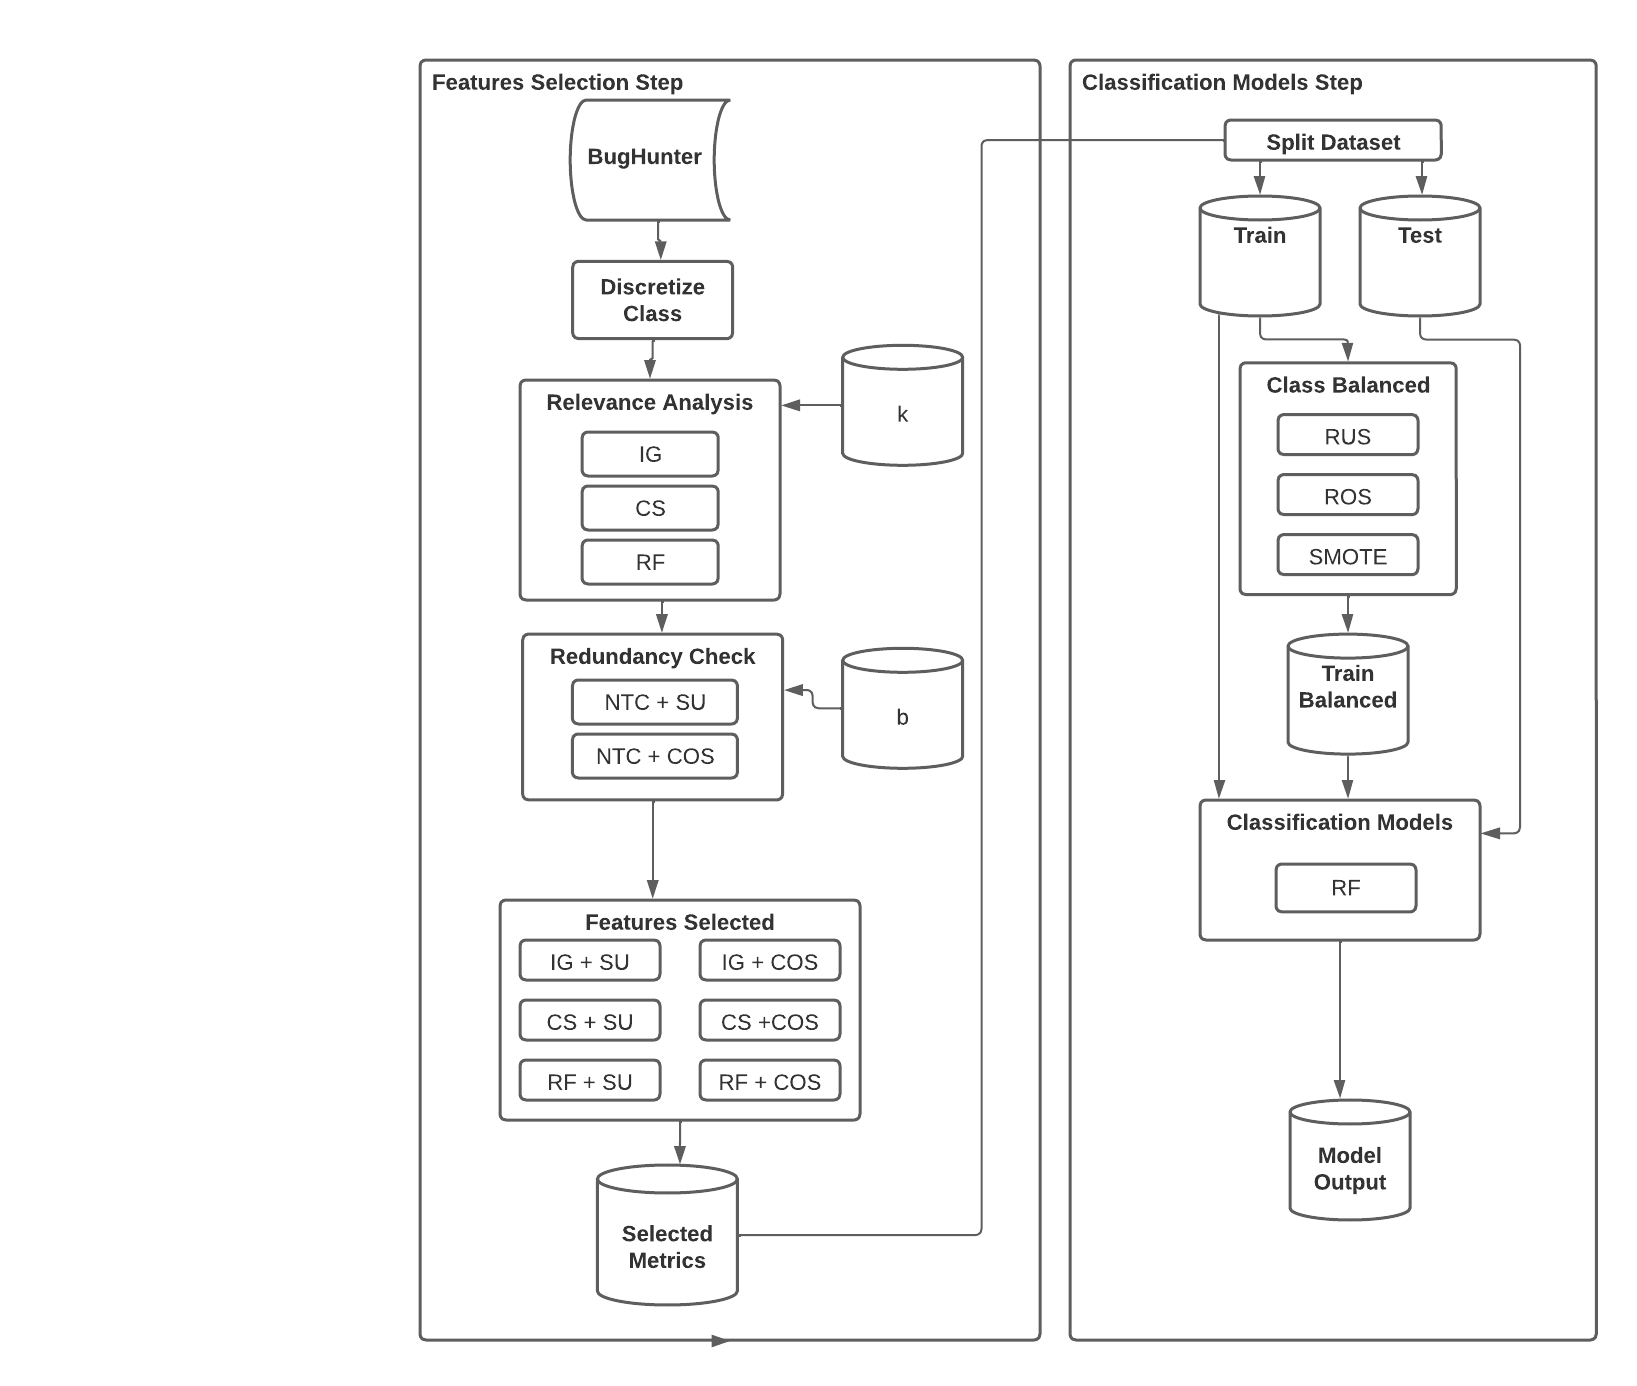
\includegraphics[width=150mm, height=110mm,]{figs/etapas/diagram.png}
    \captionsetup{labelsep=period, labelfont=bf}
    \setstretch{1} %Interlineado 1
    \caption{Descripción del flujo de trabajo}
    \label{fig:Flow}
\end{figure}

 El flujo descrito se ejecuta por cada proyecto iniciando con el proceso de selección de características. Cada proyecto contiene tres conjuntos de datos uno por cada nivel de métricas (Method, Class and File), el algoritmo \ref{alg:featureSelection} describe el primer paso del flujo \ref{fig:Flow}.
 
El algoritmo \ref{alg:featureSelection} describe el paso de Feature Selection. Se ejecuta ingresando cada conjunto de datos \(C_{p}(C_{\text{level}},C_{\text{class}},C_{\text{method}})\) donde \(_{p} \in \{p_{1},p_{2},...,p_{15}\}\) representa los 15 proyectos que contiene el BugHunter, y cada uno contiene tres conjuntos de datos, uno por cada nivel. Se guardan en la base de datos las métricas seleccionadas para cada nivel \(T_{\text{le}}(f_1,f_2,...,f_k)\) después de aplicar el análisis de relevancia y el control de redundancia. Utilizando tres ciclos anidados, se recorren las listas (\(rankList, bList, levelList\)) con la jerarquía \(rank \rightarrow \beta \rightarrow \text{level}\), donde \(rank\) se utiliza para seleccionar las métricas después del proceso de análisis de relevancia (IG, CS y RF), \(\beta\) es el umbral que se define para la ejecución del algoritmo NTC (análisis de redundancia), y \(\text{level}\) representa el nivel que se selecciona para el proyecto que se está analizando.

En cada iteración se lee el conjunto de datos (\(proyecto \rightarrow nivel\)) y se normaliza el atributo clase, dado que contiene valores numéricos que representan la cantidad de errores encontrados en esa medición, quedando solo con las clases BUG y NOBUG.

Se realiza el proceso de análisis de relevancia y el control de redundancia, y queda guardado en la base de datos qué métricas son seleccionadas en cada iteración y qué modelo de selección se utilizó, siendo este la combinación entre los algoritmos de relevancia y el control de redundancia. La lista queda como \(modelsSelections \rightarrow ['CS-SU','IG-SU','RF-SU','CS-COS','IG-COS','RF-COS']\).

 \begin{algorithm}[H]
    \hspace*{\algorithmicindent} \textbf{Input:} The original dataset $T_{le}(f_{1},f_{2},...,f_{k},l)$ where $l \in \{FP,NFP\}$ denotes the class label, and $k$ is the number of features. $le \in \{File, Class, Methods\}$ of a specific project

    \hspace*{\algorithmicindent} \textbf{Output:} Saves the selected characteristics in the Database. $T_{le}(f_1,f_2,...,f_k,l)$ where $k$ is the number of features selected by relevance analysis and redundancy check.
    \caption{Feature selection}
    \label{alg:featureSelection}
    \begin{algorithmic}[1]
    \fontsize{12pt}{12pt}\selectfont
    \REQUIRE $rankList \leftarrow [0.5, 0.7, 0.9]$
    \STATE $bList \leftarrow [0.5, 0.7, 0.9]$
    \STATE $levelList \leftarrow ['method', 'class', 'file']$
    \STATE $response \leftarrow \phi$

    \FOR{$\text{each}$ rank in $rankList$}
        \FOR{$\text{each}$ b in $bList$}
            \FOR{$\text{each}$ level in $levelList$}
                \STATE $data \leftarrow readDataset(level, project)$
                \STATE $data \leftarrow normalizeClass(data)$\;
                \STATE $square \leftarrow ChiSquare(data, rank)$\;
                \STATE $ig \leftarrow Ig(data, rank)$\;
                \STATE $relief \leftarrow ReliefF(data, rank)$\;
                \STATE $response \leftarrow response + NTC(b, square, 'CS-SU')$\;
                \STATE $response \leftarrow response + NTC(b, ig, 'IG-SU')$\;
                \STATE $response \leftarrow response + NTC(b, relief, 'RF-SU')$\;
                \STATE $response \leftarrow response + NTC(b, square, 'CS-COS')$\;
                \STATE $response \leftarrow response + NTC(b, ig, 'IG-COS')$\;
                \STATE $response \leftarrow response + NTC(b, relief, 'RF-COS')$\;
                \STATE $saveBD(response)$\;
            \ENDFOR
        \ENDFOR
    \ENDFOR
    \end{algorithmic}
\end{algorithm}

El algoritmo \ref{alg:executionmodels} representa el paso de modelos de clasificación. Se ingresan los mismos conjuntos de datos del algoritmo \ref{alg:featureSelection} pero $_{k}$ representa las métricas seleccionadas al ejecutar algoritmo \ref{alg:featureSelection}.

A los modelos de selección (\(modelsSelections\)) resultantes del algoritmo \ref{alg:executionmodels} se les agrega \(ALL\) que representa al conjunto de datos original sin realizar el paso de selección de características. Se agrega la lista de esquemas (\(modelsSelections\)) a los ciclos anidados. Quedando \(rank \rightarrow \beta \rightarrow level \rightarrow modelSelection\).

\begin{algorithm}[H]
    \hspace*{\algorithmicindent} \textbf{Input:} \\ The dataset $T_{le}(f_1, f_2, ..., f_k, l)$ where $l \in \{FP, NFP\}$ denotes the class label, and $k$ is the number of features selected by the feature selection process. $le \in \{File, Class, Methods\}$ of a specific project

    \hspace*{\algorithmicindent} \textbf{Output:} 
        Saves the precision, recall, accuracy, and f-measure in the Database 
    \caption{Execution of models}
    \label{alg:executionmodels}
    \begin{algorithmic}[1]
    \fontsize{12pt}{12pt}\selectfont
    \REQUIRE $rankList \leftarrow [0.5, 0.7, 0.9]$
    \STATE $rankList \leftarrow [0.5, 0.7, 0.9]$
    \STATE $bList \leftarrow [0.5, 0.7, 0.9]$
    \STATE $levelList \leftarrow ['method', 'class', 'file']$

    \STATE $modelsSelections \leftarrow ['CS-SU', 'IG-SU', 'RF-SU', 'CS-COS', 'IG-COS', 'RF-COS', 'ALL']$\;
    \STATE $response \leftarrow \phi$

    \FOR{$\text{each}$ rank in $rankList$}
        \FOR{$\text{each}$ b in $bList$}
            \FOR{$\text{each}$ level in $levelList$}
                \FOR{$\text{each}$ modelsSelection in $modelsSelections$}
                \STATE $data \leftarrow getData(rank, b, level, modelsSelection)$\;
                    \STATE $responseNormal \leftarrow ModelResult(data.original, model)$\;
                    \STATE $responseBalanced \leftarrow ModelResult(data.balanced, model)$\;
                    \STATE $saveBD(responseNormal)$\;
                    \STATE $saveBD(responseBalanced)$\;
                \ENDFOR
            \ENDFOR
        \ENDFOR
    \ENDFOR

    \end{algorithmic}
\end{algorithm}



En cada iteración se obtiene el conjunto de datos aplicando los filtros de métricas mencionados, este se utiliza para ejecutar los modelos de clasificación de la lista $models$. Los resultados de presision, recall y f-measure se almacenan en base de datos así como cada parámetro referente a la iteración para identificar a que conjunto de datos pertenecen y los parámetros de selección.





\section{La Medida de Rendimiento}

En el estudio principal se implementó el clasificador \textit{Random Forest} en la herramienta \textbf{Weka} \cite{weka}. Para la evaluación del modelo se utilizó la configuración \textit{Supplied Test Set}, que permite evaluar sobre un conjunto de prueba predefinido ---generado previamente en Python mediante partición estratificada 67/33---, de modo que todas las variantes de un mismo conjunto de datos se evalúan contra exactamente las mismas instancias.

El desempeño se mide con precisión, \textit{recall} y \textit{F-measure}, definidas en la Sección \ref{sec:metricas_evaluacion}. El valor de \textit{F-measure} reportado corresponde al agregado ponderado por la frecuencia de cada clase que entrega la herramienta para cada ejecución. De cada una de las ejecuciones del estudio principal se almacenaron esos valores agregados ---precisión, \textit{recall}, \textit{F-measure} y exactitud--- junto con los parámetros que identifican la configuración; no se conservaron las predicciones individuales ni las probabilidades estimadas. Las excepciones son la línea base del conjunto ``All'' a nivel de método, cuya salida completa de Weka se conservó (Tabla \ref{tab:porclase}), y las mejores configuraciones a nivel de método, de las que se conservó la matriz de confusión (Tabla \ref{table:weka_method_smote_b}). Por ello, las métricas por clase (\textit{F-measure} de la clase \textit{bug}, MCC y AUC-ROC) se obtienen de forma sistemática solo en el análisis de sensibilidad (Sección \ref{sec:sensibilidad}), diseñado para almacenarlas en todas sus ejecuciones.

El conjunto de datos tiene tres niveles de código fuente (método, clase y archivo) y 15 proyectos, además del conjunto resumido ``All''. La línea base se estableció con 2.592 ejecuciones y el estudio de selección de características y balanceo con 13.916 ejecuciones de \textit{Random Forest}; dado el tamaño de las tablas completas, se presentan los mejores resultados por proyecto y los agregados.

\section{Resultados con dataset original}
\label{sec:datasetoriginal}

En la sección actual, llevamos a cabo un experimento con el objetivo de replicar los resultados reportados en \cite{ferenc_automatically_2020}, enfocándonos en las métricas de código en distintos niveles. El estudio original aplicó once algoritmos de aprendizaje automático con cross validation de 10 folds en la herramienta WEKA sobre quince proyectos (y el dataset resumen), considerando tres niveles distintos en cada uno. En nuestro enfoque para replicar estos hallazgos, empleamos los mismos proyectos pero restringimos nuestra experimentación al algoritmo RandomForest de aprendizaje automático. Esta limitación se basó en la hipótesis de si sería posible alcanzar resultados comparables a los reportados en \cite{ferenc_automatically_2020}.

A continuación, presentamos en la Tabla \ref{table:original_result_average} una comparativa entre el promedio de nuestros resultados y los obtenidos en \cite{ferenc_automatically_2020}. Es importante señalar que, en nuestro experimento, se promediaron menos datos debido a la selección de una cantidad menor de algoritmos de aprendizaje automático para la prueba.

\begin{table}[H]
\captionsetup{labelsep=period, labelfont=bf}
\caption{\label{table:original_result_average} Resultado promedio de la medida f para nuestra investigación y el artículo que creó BugHunter }
\centering
\begin{tabular}{lll}
\toprule
       & Este trabajo       & Ferenc et al.     \\
\midrule
Nivel  & F-measure & F-measure \\
\hline
Método & 0,63      & 0,63      \\
Clase  & 0,50      & 0,56      \\
Archivo   & 0,50      & 0,54    \\
\bottomrule
\end{tabular}

\end{table}

Los resultados presentados en la Tabla \ref{table:original_result_average} revelan que, en promedio, nuestros hallazgos son comparables a pesar de haber realizado un número menor de experimentos. Esta observación nos permite afirmar, a nivel global, que hemos conseguido obtener resultados análogos a los reportados en \cite{ferenc_automatically_2020}. Tal similitud resalta la eficacia del algoritmo RandomForest en la evaluación de métricas de código en distintos niveles, y respalda la solidez del enfoque metodológico adoptado en el estudio original.

\subsection{Resultados Utilizando el Conjunto de Datos Original a Nivel de Método}
La Tabla \ref{table:original_result_weka_method_result} presenta los resultados de entrenar el modelo RandomForest con métricas a nivel de método para predecir fallos en este mismo nivel. La estructura de la tabla es la siguiente:

\begin{itemize}
  \item \textbf{Project:} Lista los proyectos de software analizados en el estudio. Cada uno representa una instancia de análisis individual y se incluye un conjunto denominado ALL, que es la unión de todos los proyectos.
  \item \textbf{F-measure:} Indica el valor de la medida F para cada proyecto, una métrica esencial en la valoración del rendimiento de modelos de aprendizaje automático, combinando precisión y recall.
\end{itemize}


\begin{table}[H]
\captionsetup{labelsep=period, labelfont=bf}
\caption{\label{table:original_result_weka_method_result} Resultados utilizando el conjunto de datos original a nivel de método}
\centering
{
\fontsize{12pt}{12pt}\selectfont
\begin{tabular}{ll}
\toprule
\multicolumn{2}{c}{MÉTODO} \\
\toprule
Proyecto                        & F-measure \\
\midrule
oryx                           & 0,852     \\
antlr4                         & 0,781     \\
BroadleafCommerce              & 0,778     \\
mct                            & 0,748     \\
junit                          & 0,695     \\
netty                          & 0,676     \\
ceylon-ide-eclipse             & 0,644     \\
titan                          & 0,584     \\
all                            & 0,579     \\
elasticsearch                  & 0,561     \\
mcMMO                          & 0,561     \\
orientdb                       & 0,56      \\
neo4j                          & 0,545     \\
hazelcast                      & 0,542     \\
MapDB                          & 0,52      \\
Android-Universal-Image-Loader & 0,486     \\
\bottomrule
\end{tabular}
}

\end{table}


El proyecto oryx obtuvo el mejor resultado a nivel de método con una F-measure de 0,85, mientras que en el estudio original de \cite{ferenc_automatically_2020}, el proyecto antlr4 mostró el mejor resultado con un valor de 0,75 \cite{ferenc_automatically_2020}. En nuestro análisis, el proyecto antlr4 alcanzó una F-measure de 0,78, lo que demuestra una similitud notable con los resultados originales. En el estudio de \cite{ferenc_automatically_2020}, el proyecto oryx tuvo una F-measure de 0,66, lo que indica la necesidad de un análisis más exhaustivo centrado en este proyecto para determinar las causas de la diferencia significativa de 0,19. Los demás proyectos mostraron valores comparables, con una variación promedio de ±0,10 en relación con los resultados del estudio original.

\begin{table}[H]
 \captionsetup{labelsep=period, labelfont=bf}
\caption{\label{table:original_result_weka_class_result} Resultados utilizando el conjunto de datos original a nivel de clase}
\centering
{
\fontsize{12pt}{10pt}\selectfont
\begin{tabular}{ll}
\toprule 
\multicolumn{2}{c}{CLASE} \\
\midrule 
Proyecto                        & F-measure \\
\hline 
oryx                           & 0,787     \\
BroadleafCommerce              & 0,687     \\
mct                            & 0,566     \\
junit                          & 0,543     \\
ceylon-ide-eclipse             & 0,533     \\
MapDB                          & 0,51      \\
all                            & 0,484     \\
hazelcast                      & 0,482     \\
elasticsearch                  & 0,481     \\
netty                          & 0,461     \\
orientdb                       & 0,456     \\
mcMMO                          & 0,446     \\
titan                          & 0,397     \\
antlr4                         & 0,387     \\
Android-Universal-Image-Loader & 0,358     \\
neo4j                          & 0,338    \\
\bottomrule
\end{tabular}
}

\end{table}


En lo que respecta a las métricas de código a nivel de clases, observamos una variación promedio de ±0,10 en todos los proyectos. Esta discrepancia podría atribuirse al uso de una mayor variedad de algoritmos de aprendizaje automático en el estudio original. No obstante, hemos conseguido resultados comparables, logrando así cumplir con nuestro objetivo inicial. Es importante resaltar que, una vez más, el proyecto oryx se posiciona a la cabeza en este nivel, mostrando una mínima diferencia de 0,08 en la F-measure en comparación con el estudio original. Este hallazgo es notable considerando que, en el análisis original a nivel de clase, el mejor desempeño lo obtuvo BroadleafCommerce con una F-measure de 0,74 utilizando el algoritmo RandomForest. Estos resultados subrayan la consistencia de oryx en nuestros experimentos y reflejan la efectividad del algoritmo RandomForest en diferentes contextos y niveles de métrica.

\begin{table}[H]
\captionsetup{labelsep=period, labelfont=bf}
\caption{\label{table:original_result_weka_file_result} Resultados utilizando el conjunto de datos original a nivel de archivo}
\centering
{
\fontsize{12pt}{10pt}\selectfont
\begin{tabular}{ll}
\toprule 
\multicolumn{2}{c}{ARCHIVO} \\
\midrule 
Proyecto                        & F-measure \\
\hline 
oryx                           & 0,77      \\
BroadleafCommerce              & 0,67      \\
mct                            & 0,586     \\
ceylon-ide-eclipse             & 0,541     \\
antlr4                         & 0,501     \\
all                            & 0,482     \\
elasticsearch                  & 0,474     \\
hazelcast                      & 0,474     \\
orientdb                       & 0,47      \\
junit                          & 0,468     \\
netty                          & 0,45      \\
mcMMO                          & 0,447     \\
MapDB                          & 0,444     \\
titan                          & 0,436     \\
neo4j                          & 0,362     \\
Android-Universal-Image-Loader & 0,344    \\
\bottomrule
\end{tabular}
}

\end{table}


Al considerar las métricas a nivel de archivo, nuevamente destacamos que el proyecto oryx obtuvo el mejor resultado con una F-measure de 0,77. Esto contrasta con los hallazgos del estudio original, donde el proyecto BroadleafCommerce lideró con una F-measure de 0,77, seguido por oryx con 0,64, lo cual representa una diferencia de 0,13 en comparación con nuestros resultados. En este nivel, también observamos una variación promedio de ±0,10 en los valores obtenidos para la F-measure.

Estos experimentos han permitido alinear nuestros resultados iniciales con aquellos reportados en el estudio original, estableciendo una base sólida para futuras mejoras. Estas mejoras se centrarán en la reducción del número de métricas utilizadas en los algoritmos de aprendizaje automático, manteniendo o incluso superando los resultados obtenidos en esta fase experimental. Para todos los proyectos, a nivel de método se introducen 72 características en los algoritmos, a nivel de clase 92, y a nivel de archivo 6. Por tanto, el objetivo será minimizar el número de características introducidas, buscando optimizar la eficacia y eficiencia de los modelos de predicción empleados.

\subsection{Desglose por clase de la línea base}

La salida completa de Weka para la línea base del conjunto ``All'' a nivel de método se conservó, lo que permite desglosar su desempeño por clase (Tabla \ref{tab:porclase}). El contraste es ilustrativo: el \textit{F-measure} ponderado de 0,565 encubre un \textit{F-measure} de solo 0,356 para la clase \textit{bug} (precisión de 0,410 y \textit{recall} de 0,314), con un MCC de 0,052 y un AUC-ROC de 0,539, valores apenas superiores a los de un clasificador aleatorio. Este desglose cuantifica de forma directa cuánto puede encubrir la métrica agregada respecto de la clase de interés práctico (Sección \ref{sec:RQ4}), y es coherente con el desempeño no superior del conjunto unificado frente a los proyectos individuales (RQ5).

\begin{table}[H]
\centering
\caption{Desglose por clase de la línea base (Weka, Random Forest, validación cruzada de 10 particiones) sobre el conjunto ``All'' a nivel de método}
\label{tab:porclase}
\begin{tabular}{lccccc}
\toprule
Clase & Precisión & \textit{Recall} & \textit{F-measure} & MCC & AUC-ROC \\
\midrule
No-bug & 0,646 & 0,735 & 0,688 & 0,052 & 0,539 \\
Bug    & 0,410 & 0,314 & 0,356 & ---   & ---   \\
\midrule
Prom. ponderado & 0,559 & 0,579 & 0,565 & 0,052 & 0,539 \\
\bottomrule
\end{tabular}
\end{table}


\section{Experimento exploratorio preliminar en Python}
\label{sec:exploratorio_python}

Antes del estudio principal se realizó un experimento exploratorio en Python, a nivel de método, con tres clasificadores (\textit{Random Forest}, árbol de decisión y Naive Bayes). Su objetivo fue examinar el efecto de aplicar el balanceo de clases antes o después de la partición en entrenamiento y prueba. Sus resultados no responden directamente a las preguntas de investigación ---que se responden con el estudio principal en Weka (Secciones \ref{sec:RQ1} a \ref{sec:RQ5})---, sino que motivaron la decisión metodológica de balancear exclusivamente el conjunto de entrenamiento. Según el código conservado, en la variante que balancea solo el entrenamiento las métricas se calcularon para la clase positiva (\textit{bug}); el tipo de promedio de la variante que balancea el conjunto completo no pudo verificarse. Se emplearon las siguientes bibliotecas:

\begin{itemize}
    \item \textbf{Pandas:} Utilizada para la manipulación y análisis de datos, facilitando la carga, procesamiento y visualización de los conjuntos de datos.
    \item \textbf{NumPy:} Empleada para operaciones matemáticas y manipulación de arreglos, complementando a Pandas en el manejo eficiente de datos numéricos.
    \item \textbf{Scikit-learn:} Biblioteca utilizada para el preprocesamiento de datos, la partición en entrenamiento y prueba y la implementación de los modelos de clasificación de este experimento.
    \item \textbf{Imbalanced-learn:} Utilizada específicamente para técnicas de balanceo de clases, incluyendo ROS (Random Over Sampling), RUS (Random Under Sampling) y SMOTE (Synthetic Minority Over-sampling Technique).
    \item \textbf{Matplotlib y Seaborn:} Empleadas para la visualización de datos y resultados, generando gráficos y figuras que facilitan la interpretación de los resultados obtenidos.
\end{itemize}

En una primera variante del experimento, las técnicas de balanceo se aplicaron al conjunto de datos completo, antes de la partición. Esto implica que tanto el conjunto de entrenamiento como el de prueba pueden contener instancias generadas artificialmente o duplicadas, según el algoritmo de balanceo utilizado; en una segunda variante, el balanceo se aplicó solo al entrenamiento.


\subsection{Consecuencias negativas de balancear el conjunto completo}

En los modelos de clasificación utilizados en los experimentos, aplicar técnicas de balanceo a todo el conjunto de datos, incluyendo tanto el conjunto de entrenamiento como el de prueba, puede acarrear varias consecuencias negativas:

\begin{itemize}
    \item \textbf{Sobreajuste (Overfitting):} La inclusión de datos artificialmente generados en el conjunto de entrenamiento puede causar que el modelo se ajuste demasiado a estos datos sintéticos, disminuyendo su capacidad para generalizar correctamente a datos nuevos y no vistos.
    \item \textbf{Evaluación Sesgada:} Si el conjunto de prueba también contiene datos balanceados artificialmente, las métricas de evaluación pueden no reflejar el rendimiento real del modelo en un entorno no balanceado. Esto podría llevar a una sobreestimación de la capacidad predictiva del modelo.
    \item \textbf{Redundancia de Datos:} Los métodos de sobrerrepresentación (ROS y SMOTE) pueden introducir múltiples copias o variaciones de los mismos datos, lo que puede redundar en una menor diversidad dentro del conjunto de datos y afectar negativamente la capacidad del modelo para aprender patrones generalizables.
    \item \textbf{Pérdida de Información:} Los métodos de subrepresentación (RUS) eliminan datos de las clases mayoritarias, lo que puede llevar a la pérdida de información valiosa y afectar la capacidad del modelo para capturar la complejidad inherente de los datos originales.
    \item \textbf{Introducción de Ruido:} Los datos sintéticos generados por SMOTE pueden introducir ruido en el conjunto de datos si las nuevas instancias no reflejan adecuadamente las características del problema real, lo que puede afectar negativamente el rendimiento del modelo.
\end{itemize}

Para mitigar estas consecuencias, es recomendable aplicar las técnicas de balanceo únicamente al conjunto de entrenamiento, manteniendo el conjunto de prueba en su estado original. Esto asegura que la evaluación del modelo refleje con mayor precisión su desempeño en condiciones reales y no sesgadas.

Las tablas presentadas a continuación resumen los resultados de ambas variantes a nivel de método.

\subsection{Resultados balanceando todo el conjunto de datos}

Los valores de esta subsección están inflados por la fuga de información descrita: el conjunto de prueba contiene instancias duplicadas o sintéticas derivadas de las del entrenamiento, por lo que no reflejan el desempeño en condiciones reales. La Tabla \ref{tab:ros_results} presenta los resultados obtenidos al aplicar la técnica de Sobremuestreo Aleatorio (ROS) al conjunto completo. El algoritmo Random Forest (RF) alcanzó una F-measure de 0.95, con una precisión de 0.9 y un recall perfecto de 1, lo que indica un rendimiento excelente bajo esta técnica. Decision Tree (DT) obtuvo un valor de F-measure idéntico, con los mismos valores de precisión y recall que RF. Por otro lado, Naive Bayes (NB) presentó una F-measure de 0.69, con una precisión de 0.56 y un recall de 0.89, siendo inferior a RF y DT pero aún así notable en términos de recall.


\begin{table}[H]
\centering
\captionsetup{labelsep=period, labelfont=bf}
\caption{Resultados de los algoritmos utilizando ROS}
\fontsize{12pt}{10pt}\selectfont
\begin{tabular}{llll}
\toprule 
\textbf{Algorithm} & \textbf{Precision} & \textbf{Recall} & \textbf{F-measure} \\ 
\midrule 
RF & 0.9 & 1 & 0.95 \\ 
DT & 0.9 & 1 & 0.95 \\ 
NB & 0.56 & 0.89 & 0.69 \\ 
\bottomrule
\end{tabular}

\label{tab:ros_results}
\end{table}



En la Tabla \ref{tab:rus_results} se muestran los resultados de los algoritmos de clasificación utilizando la técnica de Submuestreo Aleatorio (RUS). DT alcanzó una F-measure de 0.85, con una precisión de 0.93 y un recall de 0.82, mostrando un equilibrio sólido entre precisión y recall. RF obtuvo una F-measure de 0.77, con una precisión de 0.82 y un recall de 0.78, mientras que NB logró una F-measure de 0.68, con una precisión de 0.55 y un recall de 0.89, destacándose más en el recall.


\begin{table}[H]
\centering
\captionsetup{labelsep=period, labelfont=bf}
\caption{Resultados de los algoritmos utilizando RUS}
\fontsize{12pt}{10pt}\selectfont
\begin{tabular}{llll}
\toprule 
\textbf{Algorithm} & \textbf{Precision} & \textbf{Recall} & \textbf{F-measure} \\ 
\midrule 
DT & 0.93 & 0.82 & 0.85 \\ 
RF & 0.82 & 0.78 & 0.77 \\ 
NB & 0.55 & 0.89 & 0.68 \\ 
\bottomrule
\end{tabular}

\label{tab:rus_results}
\end{table}


La Tabla \ref{tab:smote_results} resume los resultados al aplicar la técnica SMOTE. El algoritmo RF obtuvo una F-measure de 0.88, con una precisión de 0.89 y un recall de 0.89, destacándose nuevamente como el mejor desempeño. DT logró una F-measure de 0.85, con una precisión de 0.87 y un recall de 0.83, siendo ligeramente inferior a RF. NB presentó una F-measure de 0.70, con una precisión de 0.56 y un recall de 0.92, mostrando una vez más un alto recall.


\begin{table}[H]
\centering
\captionsetup{labelsep=period, labelfont=bf}
\caption{Resultados de los algoritmos utilizando SMOTE}
\fontsize{12pt}{10pt}\selectfont
\begin{tabular}{llll}
\toprule 
\textbf{Algorithm} & \textbf{Precision} & \textbf{Recall} & \textbf{F-measure} \\ 
\midrule 
RF & 0.89 & 0.89 & 0.88 \\ 
DT & 0.87 & 0.83 & 0.85 \\ 
NB & 0.56 & 0.92 & 0.70 \\ 
\bottomrule
\end{tabular}

\label{tab:smote_results}
\end{table}


Los resultados sin aplicar ninguna técnica de balanceo se presentan en la Tabla \ref{tab:none_results}. NB mostró una F-measure de 0.47, con una precisión de 0.37 y un recall de 0.76, mientras que RF obtuvo una F-measure de 0.40, con una precisión de 0.49 y un recall de 0.35. DT alcanzó una F-measure de 0.42, con una precisión de 0.43 y un recall de 0.41. Estos resultados reflejan el impacto negativo del desequilibrio de clases en el rendimiento de los algoritmos, con un notable descenso en la precisión.

\begin{table}[H]
\centering
\captionsetup{labelsep=period, labelfont=bf}
\caption{Resultados de los algoritmos sin técnicas de balanceo}
\fontsize{12pt}{10pt}\selectfont
\begin{tabular}{llll}
\toprule 
\textbf{Algorithm} & \textbf{Precision} & \textbf{Recall} & \textbf{F-measure} \\ 
\midrule 
NB & 0.37 & 0.76 & 0.47 \\ 
DT & 0.43 & 0.41 & 0.42 \\ 
RF & 0.49 & 0.35 & 0.40 \\ 
\bottomrule
\end{tabular}

\label{tab:none_results}
\end{table}


Finalmente, la Tabla \ref{tab:best_f_measure} proporciona una visión general de los mejores valores de F-measure obtenidos por diferentes proyectos a nivel de método. El proyecto ``oryx'' alcanzó la F-measure más alta de 0.88 utilizando RF, seguido de ``antlr4'' con una F-measure de 0.87 también con RF. En términos de precisión y recall, ``oryx'' mostró una precisión de 0.89 y un recall de 0.89, mientras que ``antlr4'' tuvo una precisión de 0.87 y un recall de 0.83. En contraste, los proyectos ``mct'' y ``BroadleafCommerce'' lograron F-measures de 0.82 y 0.78 respectivamente, utilizando RF, con valores de precisión y recall consistentes. ``junit'' y ``netty'' obtuvieron F-measures de 0.77 y 0.72 respectivamente, también utilizando RF, manteniendo un equilibrio adecuado entre precisión y recall.

\begin{table}[H]
\centering
\captionsetup{labelsep=period, labelfont=bf}
\caption{Los mejores valores de F-measure por proyecto a nivel de método}
\fontsize{12pt}{10pt}\selectfont
\begin{tabular}{lll}
\toprule 
\textbf{Project} & \textbf{F-measure} & \textbf{Algorithm} \\ \midrule 
oryx & 0.88 & RF \\ 
antlr4 & 0.87 & RF \\ 
mct & 0.82 & RF \\ 
BroadleafCommerce & 0.78 & RF \\ 
junit & 0.77 & RF \\ 
netty & 0.72 & RF \\ 
titan & 0.72 & RF \\ 
ceylon-ide-eclipse & 0.71 & RF \\ 
mcMMO & 0.66 & NB \\ 
elasticsearch & 0.62 & NB \\ 
\bottomrule
\end{tabular}

\label{tab:best_f_measure}
\end{table}


\subsection{Resultados balanceando solo conjunto de datos de entrenamiento}

Buscando mitigar las consecuencias negativas descritas anteriormente, se realizan nuevos experimentos balanceando solo el conjunto de datos de entrenamiento evitando la posibilidad de que existan datos generados o duplicados en el conjunto de pruebas.

\subsubsection{Resultados Utilizando ROS}
La Tabla \ref{tab:results_ros_sin} presenta los resultados de aplicar el algoritmo ROS (Random Over Sampling) únicamente al conjunto de datos de entrenamiento. Este método incrementa artificialmente el número de instancias de la clase minoritaria mediante duplicación. Los resultados muestran que el modelo Naive Bayes (NB) alcanzó una precisión de 0.37, un recall de 0.97 y una F-measure de 0.54. Este alto valor de recall indica que el modelo es efectivo en identificar la mayoría de las instancias de la clase minoritaria, aunque a costa de una baja precisión, lo que sugiere muchos falsos positivos. El Random Forest (RF) y el Decision Tree (DT) mostraron un desempeño más equilibrado en términos de precisión y recall, aunque con valores más bajos comparados con NB. RF alcanzó una precisión de 0.53, un recall de 0.48 y una F-measure de 0.50, mientras que DT mostró una precisión de 0.38, un recall de 0.60 y una F-measure de 0.46.


\begin{table}[H]
\centering
\caption{Resultado de los algoritmos utilizando ROS con balanceo solo al conjunto de entrenamiento}
\captionsetup{labelsep=period, labelfont=bf}
\fontsize{12pt}{10pt}\selectfont
\begin{tabular}{lccc}
\toprule 
\textbf{Modelo} & \textbf{Precisión} & \textbf{Recall} & \textbf{F-measure} \\
\midrule  
NB & 0.37 & 0.97 & 0.54 \\
RF & 0.53 & 0.48 & 0.50 \\
DT & 0.38 & 0.60 & 0.46 \\
\bottomrule
\end{tabular}
\label{tab:results_ros_sin}
\end{table}


\subsubsection{Resultados Utilizando RUS}
La Tabla \ref{tab:results_rus_sin} muestra los resultados de aplicar el algoritmo RUS (Random Under Sampling) solo al conjunto de entrenamiento. Este método reduce el número de instancias de la clase mayoritaria para equilibrar el dataset. Los resultados indican que NB mantiene su rendimiento con una precisión de 0.37, un recall de 0.97 y una F-measure de 0.54. Sin embargo, se observan mejoras en RF y DT comparados con los resultados obtenidos con ROS. RF mejora su precisión a 0.43 y su recall a 0.59, obteniendo una F-measure de 0.50, mientras que DT mejora en precisión a 0.43 y en recall a 0.58, logrando una F-measure de 0.49. Esto sugiere que RUS puede ser más efectivo que ROS para estos algoritmos al mejorar la representación de la clase minoritaria sin introducir demasiados falsos positivos.


\begin{table}[H]
\centering
\captionsetup{labelsep=period, labelfont=bf}
\caption{Resultado de los algoritmos utilizando RUS con balanceo solo al conjunto de entrenamiento}
\fontsize{12pt}{10pt}\selectfont
\begin{tabular}{lccc}
\toprule 
\textbf{Algorithm} & \textbf{Precisión} & \textbf{Recall} & \textbf{F-measure} \\
\midrule 
NB & 0.37 & 0.97 & 0.54 \\
RF & 0.43 & 0.59 & 0.50 \\
DT & 0.43 & 0.58 & 0.49 \\
\bottomrule
\end{tabular}
\label{tab:results_rus_sin}
\end{table}




\subsubsection{Resultados Utilizando SMOTE}

La Tabla \ref{tab:results_smote_sin} detalla los resultados de utilizar SMOTE (Synthetic Minority Over-sampling Technique) para balancear el conjunto de entrenamiento. SMOTE genera nuevas instancias sintéticas de la clase minoritaria mediante interpolación. En este caso, DT muestra una notable mejora con una precisión de 0.50, un recall de 0.80 y una F-measure de 0.62. RF también mejora, alcanzando una precisión de 0.44, un recall de 0.80 y una F-measure de 0.57. NB, sin embargo, mantiene sus valores constantes con una precisión de 0.37, un recall de 0.97 y una F-measure de 0.54. Comparados con la Tabla \ref{tab:none_results} (sin balanceo), estos resultados muestran que balancear solo el entrenamiento eleva sobre todo el \textit{recall} de la clase \textit{bug}, a costa de la precisión. Es el mismo intercambio que el estudio principal y el análisis de sensibilidad cuantifican de forma sistemática (Secciones \ref{sec:RQ4} y \ref{sec:sensibilidad}).

La comparación entre ambas variantes ---valores de \textit{F-measure} de hasta 0,95 balanceando el conjunto completo frente a valores de entre 0,46 y 0,62 balanceando solo el entrenamiento--- ilustra la magnitud del sesgo que introduce balancear antes de la partición, y justifica que en el resto de la tesis el balanceo se aplique exclusivamente sobre el conjunto de entrenamiento.


\begin{table}[H]
\centering
\captionsetup{labelsep=period, labelfont=bf}
\caption{Resultado de los algoritmos utilizando SMOTE con balanceo solo al conjunto de entrenamiento}
\fontsize{12pt}{10pt}\selectfont
\begin{tabular}{lccc}
\hline
\textbf{Modelo} & \textbf{Precisión} & \textbf{Recall} & \textbf{F-measure} \\
\hline
DT & 0.50 & 0.80 & 0.62 \\
RF & 0.44 & 0.80 & 0.57 \\
NB & 0.37 & 0.97 & 0.54 \\
\hline
\end{tabular}

\label{tab:results_smote_sin}
\end{table}




En esta sección se estudian las cinco preguntas de investigación a partir de los resultados experimentales. La discusión de los hallazgos y las amenazas a la validez se presentan en el Capítulo \ref{cap:discusion}.

\section{Primera pregunta de investigación}
La primera pregunta de investigación a responder es:
\label{sec:RQ1}

\noindent\fbox{%
\parbox{\dimexpr\textwidth-2\fboxsep-2\fboxrule\relax}{%
\textbf{RQ1} ¿El análisis de relevancia y control de redundancia de características puede mejorar la identificación de bugs basado en métricas de código?%
}%
}
\vspace{12pt}

Para abordar la pregunta de investigación \textbf{RQ1} se condujo un experimento de 13.916 ejecuciones del clasificador \textit{Random Forest}. Cada conjunto proyecto-nivel se recorrió (Figura \ref{fig:Flow}) a través del espacio de parámetros definido por el umbral de relevancia (\textit{Rank}), el umbral de redundancia $\beta$ y el esquema de selección. En cada iteración se generaron en Python un conjunto de prueba con el 33\,\% de los datos, mediante partición estratificada, y dos conjuntos de entrenamiento: uno con la distribución de clases original y otro balanceado con ROS, RUS o SMOTE, técnicas aplicadas exclusivamente sobre el entrenamiento. Ambos conjuntos de entrenamiento se utilizaron para entrenar \textit{Random Forest} en la plataforma \textit{Weka}, en la modalidad \textit{Supplied test set}, evaluando siempre contra el mismo conjunto de prueba, lo que permite una comparación directa de su rendimiento. La consistencia de este flujo con una implementación equivalente en \textit{scikit-learn} se verifica en la Sección \ref{sec:validacion_flujos}.

Comparamos los resultados obtenidos con la selección de características con los resultados base obtenidos sin selección de características en la sección anterior. 

\subsection{Método}
 A nivel de método, los mejores resultados se obtienen con el proyecto Oryx, que alcanza una medida F de 0,838 y 0,837, sin balancear y balanceando las clases, respectivamente. Estos resultados se logran con 29 y 4 características, respectivamente, lo que supone una reducción del 59,7 \% y del 94,4 \% respecto a las 72 características que se usan en los resultados base. Los resultados base muestran que el proyecto Oryx tiene una medida F de 0,852, por lo que la diferencia con la selección de características es de solo 0,014. Esto indica que la selección de características permite mantener un rendimiento similar al de los resultados base, pero con una reducción significativa de la dimensionalidad de los datos. Además, esto sugiere que muchas de las características originales podrían ser irrelevantes o redundantes para la predicción de defectos de software. 

La tabla \ref{table:b_u_c_m} resume los resultados a nivel de método. 
\begin{table}[H]
{
\fontsize{6pt}{6pt}\selectfont
 \captionsetup{labelsep=period, labelfont=bf}
 \caption{\label{table:b_u_c_m} Mejor resultado por proyecto con la clase balanceada y no balanceada a nivel de método}
\centering
\resizebox{\textwidth}{!}{%
\begin{tabular}{lllllllll}
\toprule
Project                        & Rank & \beta   & Model Selection & Precision & Recall & FMeasure & Balanceado & Metrics Count \\
\midrule
Android-Universal-Image-Loader & 0,5  & 0,7 & IG\_SU         & 0,545     & 0,543  & 0,544    & VERDADERO  & 19           \\
 & 0,5  & 0,7 & RF\_COS        & 0,531     & 0,566  & 0,543    & FALSO      & 29           \\
BroadleafCommerce              & 0,5  & 0,5 & CS\_COS        & 0,757     & 0,77   & 0,762    & VERDADERO  & 35           \\
             & 0,9  & 0,5 & IG\_SU         & 0,758     & 0,777  & 0,762    & FALSO      & 28           \\
MapDB                          & 0,7  & 0,5 & IG\_SU         & 0,529     & 0,557  & 0,538    & FALSO      & 22           \\
                        & 0,9  & 0,7 & CS\_COS        & 0,52      & 0,531  & 0,525    & VERDADERO  & 64           \\
all                            & 0,9  & 0,9 & RF\_COS        & 0,567     & 0,59   & 0,573    & FALSO      & 64           \\
                            & 0,5  & 0,5 & RF\_COS        & 0,564     & 0,58   & 0,57     & VERDADERO  & 33           \\
antlr4                         & 0,5  & 0,9 & RF\_COS        & 0,8       & 0,795  & 0,797    & VERDADERO  & 29           \\
                       & 0,9  & 0,5 & IG\_COS        & 0,757     & 0,808  & 0,778    & FALSO      & 64           \\
ceylon-ide-eclipse             & 0,7  & 0,7 & IG\_COS        & 0,601     & 0,657  & 0,62     & FALSO      & 50           \\
            & 0,7  & 0,9 & IG\_COS        & 0,603     & 0,63   & 0,615    & VERDADERO  & 50           \\
elasticsearch                  & 0,5  & 0,9 & CS\_COS        & 0,567     & 0,586  & 0,571    & FALSO      & 26           \\
                & 0,5  & 0,5 & RF\_COS        & 0,561     & 0,57   & 0,564    & VERDADERO  & 35           \\
hazelcast                      & 0,7  & 0,7 & CS\_COS        & 0,551     & 0,559  & 0,553    & FALSO      & 50           \\
                     & 0,7  & 0,7 & CS\_COS        & 0,549     & 0,552  & 0,55     & VERDADERO  & 50           \\
junit                          & 0,9  & 0,9 & IG\_COS        & 0,676     & 0,722  & 0,694    & FALSO      & 64           \\
                         & 0,9  & 0,5 & CS\_COS        & 0,68      & 0,692  & 0,686    & VERDADERO  & 64           \\
mcMMO                          & 0,7  & 0,9 & IG\_COS        & 0,577     & 0,604  & 0,581    & FALSO      & 50           \\
                         & 0,7  & 0,9 & IG\_SU         & 0,575     & 0,582  & 0,578    & VERDADERO  & 10           \\
mct                            & 0,7  & 0,7 & IG\_SU         & 0,706     & 0,694  & 0,7      & FALSO      & 18           \\
                           & 0,9  & 0,9 & RF\_SU         & 0,716     & 0,667  & 0,684    & VERDADERO  & 33           \\
neo4j                          & 0,9  & 0,7 & RF\_COS        & 0,538     & 0,577  & 0,552    & FALSO      & 64           \\
                        & 0,5  & 0,9 & RF\_COS        & 0,545     & 0,555  & 0,55     & VERDADERO  & 25           \\
netty                          & 0,9  & 0,9 & RF\_COS        & 0,638     & 0,684  & 0,653    & FALSO      & 64           \\
                          & 0,7  & 0,5 & IG\_SU         & 0,636     & 0,676  & 0,651    & VERDADERO  & 10           \\
orientdb                       & 0,7  & 0,5 & RF\_COS        & 0,557     & 0,598  & 0,569    & FALSO      & 43           \\
                      & 0,5  & 0,9 & IG\_SU         & 0,561     & 0,572  & 0,566    & VERDADERO  & 6            \\
oryx                           & 0,7  & 0,7 & CS\_SU         & 0,825     & 0,859  & 0,838    & FALSO      & 29           \\
                           & 0,5  & 0,7 & IG\_SU         & 0,826     & 0,852  & 0,837    & VERDADERO  & 4            \\
titan                          & 0,7  & 0,7 & CS\_SU         & 0,634     & 0,663  & 0,645    & FALSO      & 32           \\
                        & 0,7  & 0,7 & RF\_SU         & 0,633     & 0,612  & 0,621    & VERDADERO  & 32     \\
                        \bottomrule
\end{tabular}%
}}

\end{table}

\subsection{Clase}
A nivel de clase, el proyecto Oryx también obtiene los mejores resultados, con una medida F de 0,78 tanto sin balancear como balanceando las clases. Sin embargo, la selección de características permite reducir el número de características de 92 a 6 y 47, respectivamente. Esto implica una reducción del 93,5 \% y del 48,9 \% respecto a los resultados base, que usan todas las características. Por lo tanto, la selección de características también es beneficiosa a nivel de clase, ya que permite simplificar el modelo sin perder rendimiento.
La tabla \ref{table:b_u_c_c} resume los resultados a nivel de clase.

\begin{table}[H]
{
\fontsize{6pt}{6pt}\selectfont
 \captionsetup{labelsep=period, labelfont=bf}
 \caption{\label{table:b_u_c_c} Mejor resultado por proyecto con la clase equilibrada y desequilibrada a nivel de clase}
\centering
\resizebox{\textwidth}{!}{%
\begin{tabular}{lllllllll}
\toprule
\multicolumn{1}{c}{\textbf{Project}} & \multicolumn{1}{c}{\textbf{Rank}} & \multicolumn{1}{c}{\textbf{\beta}} & \multicolumn{1}{c}{\textbf{ModelSelection}} & \multicolumn{1}{c}{\textbf{Precision}} & \multicolumn{1}{c}{\textbf{Recall}} & \multicolumn{1}{c}{\textbf{FMeasure}} & \multicolumn{1}{c}{\textbf{Balanceado}} & \multicolumn{1}{c}{\textbf{MetricsCount}} \\
\midrule
Android-Universal-Image-Loader       & 0,5                               & 0,9                            & RF\_SU                                      & 0,462                                  & 0,459                               & 0,46                                  & VERDADERO                               & 25                                        \\
       & 0,5                               & 0,9                            & RF\_COS                                     & 0,443                                  & 0,459                               & 0,448                                 & FALSO                                   & 32                                        \\
BroadleafCommerce                    & 0,5                               & 0,5                            & RF\_COS                                     & 0,701                                  & 0,701                               & 0,701                                 & FALSO                                   & 47                                        \\
                   & 0,7                               & 0,7                            & RF\_SU                                      & 0,701                                  & 0,701                               & 0,701                                 & VERDADERO                               & 48                                        \\
MapDB                                & 0,7                               & 0,9                            & IG\_SU                                      & 0,564                                  & 0,565                               & 0,563                                 & FALSO                                   & 9                                         \\
                                & 0,7                               & 0,5                            & RF\_SU                                      & 0,538                                  & 0,538                               & 0,538                                 & VERDADERO                               & 58                                        \\
all                                  & 0,5                               & 0,5                            & IG\_SU                                      & 0,528                                  & 0,53                                & 0,522                                 & VERDADERO                               & 15                                        \\
                                  & 0,7                               & 0,7                            & IG\_SU                                      & 0,521                                  & 0,523                               & 0,52                                  & FALSO                                   & 18                                        \\
antlr4                               & 0,5                               & 0,5                            & IG\_COS                                     & 0,515                                  & 0,542                               & 0,524                                 & FALSO                                   & 47                                        \\
                               & 0,5                               & 0,7                            & RF\_SU                                      & 0,517                                  & 0,517                               & 0,517                                 & VERDADERO                               & 43                                        \\
ceylon-ide-eclipse                   & 0,5                               & 0,9                            & CS\_SU                                      & 0,57                                   & 0,594                               & 0,578                                 & VERDADERO                               & 11                                        \\
                   & 0,7                               & 0,9                            & IG\_SU                                      & 0,57                                   & 0,602                               & 0,578                                 & FALSO                                   & 8                                         \\
elasticsearch                        & 0,5                               & 0,9                            & CS\_COS                                     & 0,514                                  & 0,514                               & 0,514                                 & VERDADERO                               & 11                                        \\
                       & 0,5                               & 0,9                            & CS\_COS                                     & 0,511                                  & 0,511                               & 0,511                                 & FALSO                                   & 11                                        \\
hazelcast                            & 0,5                               & 0,5                            & IG\_SU                                      & 0,52                                   & 0,517                               & 0,517                                 & FALSO                                   & 17                                        \\
                            & 0,5                               & 0,5                            & IG\_SU                                      & 0,522                                  & 0,517                               & 0,517                                 & VERDADERO                               & 17                                        \\
junit                                & 0,5                               & 0,7                            & CS\_SU                                      & 0,741                                  & 0,75                                & 0,741                                 & VERDADERO                               & 26                                        \\
                                & 0,5                               & 0,7                            & CS\_SU                                      & 0,731                                  & 0,741                               & 0,73                                  & FALSO                                   & 26                                        \\
mcMMO                                & 0,7                               & 0,9                            & IG\_SU                                      & 0,523                                  & 0,519                               & 0,521                                 & FALSO                                   & 30                                        \\
                                & 0,5                               & 0,9                            & RF\_SU                                      & 0,526                                  & 0,516                               & 0,519                                 & VERDADERO                               & 29                                        \\
mct                                  & 0,7                               & 0,9                            & RF\_SU                                      & 0,639                                  & 0,667                               & 0,648                                 & FALSO                                   & 27                                        \\
                                  & 0,9                               & 0,9                            & CS\_COS                                     & 0,609                                  & 0,625                               & 0,616                                 & VERDADERO                               & 85                                        \\
neo4j                                & 0,5                               & 0,9                            & RF\_SU                                      & 0,46                                   & 0,479                               & 0,462                                 & VERDADERO                               & 2                                         \\
                                & 0,5                               & 0,9                            & RF\_SU                                      & 0,46                                   & 0,485                               & 0,461                                 & FALSO                                   & 2                                         \\
netty                                & 0,9                               & 0,9                            & IG\_SU                                      & 0,511                                  & 0,532                               & 0,517                                 & FALSO                                   & 5                                         \\
                                & 0,5                               & 0,9                            & IG\_SU                                      & 0,512                                  & 0,517                               & 0,514                                 & VERDADERO                               & 4                                         \\
orientdb                             & 0,5                               & 0,7                            & IG\_SU                                      & 0,547                                  & 0,554                               & 0,545                                 & VERDADERO                               & 6                                         \\
                             & 0,5                               & 0,7                            & IG\_SU                                      & 0,549                                  & 0,556                               & 0,545                                 & FALSO                                   & 6                                         \\
oryx                                 & 0,5                               & 0,7                            & IG\_SU                                      & 0,757                                  & 0,818                               & 0,786                                 & FALSO                                   & 6                                         \\
                                 & 0,5                               & 0,9                            & IG\_COS                                     & 0,772                                  & 0,79                                & 0,78                                  & VERDADERO                               & 47                                        \\
titan                                & 0,7                               & 0,9                            & CS\_SU                                      & 0,473                                  & 0,473                               & 0,473                                 & FALSO                                   & 11                                        \\
                                & 0,7                               & 0,9                            & CS\_SU                                      & 0,48                                   & 0,467                               & 0,472                                 & VERDADERO                               & 11        \\
                                \bottomrule
\end{tabular}%
}}


\end{table}
\subsection{Archivo}
A nivel de archivo, el proyecto Oryx vuelve a obtener los mejores resultados, con una medida F de 0,806 con la selección de características y sin balancear las clases (0,777 balanceando). Este resultado mejora en 0,036 el resultado base, que tiene una medida F de 0,770 con todas las características. Además, la selección de características permite reducir el número de características de 6 a 3, lo que supone una reducción del 50\,\%. Así, la selección de características mejora el rendimiento y la simplicidad del modelo a nivel de archivo.

La tabla \ref{table:b_u_c_f} resume los resultados a nivel de archivo.
\begin{table}[H]
{
\fontsize{6pt}{6pt}\selectfont
\captionsetup{labelsep=period, labelfont=bf}
\caption{\label{table:b_u_c_f} Mejor resultado por proyecto con la clase balanceada y no balanceada a nivel de archivo}
\centering
\resizebox{\textwidth}{!}{%
\begin{tabular}{lllllllll}
\toprule
\multicolumn{1}{c}{\textbf{Project}} & \multicolumn{1}{c}{\textbf{Rank}} & \multicolumn{1}{c}{\textbf{\beta}} & \multicolumn{1}{c}{\textbf{ModelSelection}} & \multicolumn{1}{c}{\textbf{Precision}} & \multicolumn{1}{c}{\textbf{Recall}} & \multicolumn{1}{c}{\textbf{FMeasure}} & \multicolumn{1}{c}{\textbf{Balanceado}} & \multicolumn{1}{c}{\textbf{MetricsCount}} \\
\midrule
Android-Universal-Image-Loader       & 0,5                               & 0,5                            & CS\_SU                                      & 0,544                                  & 0,544                               & 0,544                                 & VERDADERO                               & 2                                         \\
       & 0,5                               & 0,5                            & IG\_SU                                      & 0,539                                  & 0,544                               & 0,541                                 & FALSO                                   & 2                                         \\
BroadleafCommerce                    & 0,7                               & 0,9                            & IG\_COS                                     & 0,667                                  & 0,667                               & 0,667                                 & VERDADERO                               & 4                                         \\
                    & 0,7                               & 0,9                            & IG\_COS                                     & 0,661                                  & 0,661                               & 0,661                                 & FALSO                                   & 4                                         \\
MapDB                                & 0,5                               & 0,5                            & CS\_SU                                      & 0,456                                  & 0,456                               & 0,456                                 & FALSO                                   & 3                                         \\
                                & 0,5                               & 0,5                            & IG\_COS                                     & 0,448                                  & 0,451                               & 0,449                                 & VERDADERO                               & 3                                         \\
all                                  & 0,5                               & 0,5                            & IG\_COS                                     & 0,526                                  & 0,525                               & 0,525                                 & FALSO                                   & 3                                         \\
                                  & 0,7                               & 0,7                            & CS\_COS                                     & 0,519                                  & 0,518                               & 0,518                                 & VERDADERO                               & 2                                         \\
antlr4                               & 0,7                               & 0,5                            & IG\_COS                                     & 0,557                                  & 0,548                               & 0,551                                 & VERDADERO                               & 4                                         \\
                               & 0,7                               & 0,5                            & IG\_COS                                     & 0,527                                  & 0,524                               & 0,525                                 & FALSO                                   & 4                                         \\
ceylon-ide-eclipse                   & 0,5                               & 0,9                            & IG\_COS                                     & 0,573                                  & 0,605                               & 0,578                                 & FALSO                                   & 3                                         \\
                  & 0,9                               & 0,7                            & CS\_SU                                      & 0,575                                  & 0,574                               & 0,575                                 & VERDADERO                               & 3                                         \\
elasticsearch                        & 0,5                               & 0,5                            & IG\_COS                                     & 0,518                                  & 0,519                               & 0,517                                 & FALSO                                   & 3                                         \\
                        & 0,9                               & 0,5                            & RF\_SU                                      & 0,514                                  & 0,514                               & 0,514                                 & VERDADERO                               & 2                                         \\
hazelcast                            & 0,5                               & 0,5                            & RF\_SU                                      & 0,513                                  & 0,518                               & 0,515                                 & FALSO                                   & 2                                         \\
                            & 0,9                               & 0,5                            & IG\_SU                                      & 0,512                                  & 0,514                               & 0,513                                 & VERDADERO                               & 2                                         \\
junit                                & 0,7                               & 0,7                            & CS\_COS                                     & 0,55                                   & 0,552                               & 0,547                                 & VERDADERO                               & 2                                         \\
                                & 0,7                               & 0,7                            & CS\_COS                                     & 0,506                                  & 0,507                               & 0,505                                 & FALSO                                   & 2                                         \\
mcMMO                                & 0,5                               & 0,5                            & IG\_SU                                      & 0,552                                  & 0,557                               & 0,554                                 & VERDADERO                               & 3                                         \\
                                & 0,9                               & 0,7                            & CS\_COS                                     & 0,549                                  & 0,56                                & 0,551                                 & FALSO                                   & 4                                         \\
mct                                  & 0,9                               & 0,7                            & RF\_SU                                      & 0,6                                    & 0,6                                 & 0,6                                   & FALSO                                   & 4                                         \\
                                  & 0,7                               & 0,7                            & RF\_SU                                      & 0,6                                    & 0,6                                 & 0,6                                   & VERDADERO                               & 4                                         \\
neo4j                                & 0,9                               & 0,7                            & RF\_SU                                      & 0,462                                  & 0,462                               & 0,462                                 & FALSO                                   & 2                                         \\
                                & 0,5                               & 0,7                            & IG\_COS                                     & 0,456                                  & 0,455                               & 0,456                                 & VERDADERO                               & 2                                         \\
netty                                & 0,5                               & 0,7                            & IG\_COS                                     & 0,519                                  & 0,524                               & 0,521                                 & VERDADERO                               & 3                                         \\
                                & 0,7                               & 0,7                            & CS\_COS                                     & 0,506                                  & 0,51                                & 0,508                                 & FALSO                                   & 2                                         \\
orientdb                             & 0,5                               & 0,9                            & IG\_COS                                     & 0,567                                  & 0,569                               & 0,564                                 & VERDADERO                               & 3                                         \\
                             & 0,5                               & 0,9                            & IG\_COS                                     & 0,571                                  & 0,572                               & 0,563                                 & FALSO                                   & 3                                         \\
oryx                                 & 0,5                               & 0,5                            & IG\_COS                                     & 0,784                                  & 0,836                               & 0,806                                 & FALSO                                   & 3                                         \\
                                 & 0,5                               & 0,5                            & CS\_COS                                     & 0,796                                  & 0,761                               & 0,777                                 & VERDADERO                               & 3                                         \\
titan                                & 0,5                               & 0,5                            & CS\_COS                                     & 0,452                                  & 0,466                               & 0,457                                 & FALSO                                   & 2                                         \\
                                & 0,5                               & 0,5                            & CS\_COS                                     & 0,433                                  & 0,441                               & 0,436                                 & VERDADERO                               & 2                                        
\\\bottomrule
\end{tabular}%
}
}

\end{table}

\subsection{Resultados agregados sobre los 15 proyectos}

El patrón observado en Oryx se confirma al agregar los 15 proyectos individuales (Tabla \ref{tab:agg}): la mediana del mejor \textit{F-measure} apenas varía entre las versiones sin balancear y balanceada en los tres niveles, con reducciones medianas del número de características del 40\,\% a nivel de método, 88\,\% a nivel de clase y 50\,\% a nivel de archivo. En cuanto a los esquemas, la Semejanza de Coseno (COS) predominó en el control de redundancia a nivel de método y archivo, mientras que la Incertidumbre Simétrica (SU) fue más frecuente a nivel de clase.

\begin{table}[H]
\centering
\caption{Mejor \textit{F-measure} por proyecto agregado sobre los 15 proyectos individuales (mediana [mín--máx])}
\label{tab:agg}
\begin{tabular}{lcc}
\toprule
Nivel & Sin balancear & Balanceado \\
\midrule
Método  & 0,620 [0,538--0,838] & 0,615 [0,525--0,837] \\
Clase   & 0,524 [0,448--0,786] & 0,519 [0,460--0,780] \\
Archivo & 0,525 [0,456--0,806] & 0,547 [0,436--0,777] \\
\bottomrule
\end{tabular}
\end{table}

\textit{Advertencia sobre el sesgo de comparar el mejor esquema contra una única configuración de referencia.} Las Tablas \ref{table:b_u_c_m}, \ref{table:b_u_c_c}, \ref{table:b_u_c_f} y \ref{tab:agg} comparan el mejor esquema de selección ---un máximo sobre las 54 combinaciones de algoritmo de relevancia, medida de redundancia, \textit{Rank} y $\beta$--- frente a una única configuración de referencia (todas las características). Esta comparación introduce una asimetría optimista estructural que, a diferencia de lo que ocurre en RQ4, no se cancela con una comparación simétrica. Por ello, la evidencia más robusta de RQ1 corresponde a las medianas de la Tabla \ref{tab:agg} y a las del análisis de sensibilidad (Sección \ref{sec:sensibilidad}), antes que a la cifra máxima de 94\,\% obtenida en una única celda (proyecto Oryx, nivel método). La eliminación completa de este sesgo, seleccionando el esquema sobre una partición de validación independiente de la de prueba, se declara como trabajo futuro (Capítulo \ref{cap:conclusion}).


\noindent\fbox{%
\parbox{\dimexpr\textwidth-2\fboxsep-2\fboxrule\relax}{%
\textbf{Respuesta RQ1} Los hallazgos experimentales corroboran la eficacia de las estrategias implementadas para el análisis de relevancia y la mitigación de redundancia, las cuales han facilitado una compresiva reducción de características manteniendo la integridad de los resultados iniciales. Específicamente, el algoritmo de \textit{Semejanza de Coseno} (COS) se identificó como preponderante para el nivel de método y archivo, mientras que la \textit{Incertidumbre Simétrica} (SU) fue preeminente a nivel de clases. Estas técnicas reducen la mediana del número de métricas en un 40\,\%, 88\,\% y 50\,\% en los niveles de método, clase y archivo, respectivamente (hasta un 94\,\% en el mejor caso individual), con una pérdida de \textit{F-measure} inferior a 0,02. El análisis de sensibilidad (Sección \ref{sec:sensibilidad}) confirma que este resultado se mantiene con XGBoost y SVM lineal.

}%
}
\vspace{12pt}





\section{Segunda pregunta de investigación}
\label{sec:RQ2}

\noindent\fbox{%
\parbox{\dimexpr\textwidth-2\fboxsep-2\fboxrule\relax}{%
\textbf{RQ2} ¿Cuales métricas de código fuente son buenas predictoras de errores y en que tipo de métrica (archivo, clase,
método) proporciona mejores resultados?%
}%
}
\vspace{12pt}

Se implementaron 6 algoritmos de selección de características (\ref{fig:Flow}) y al terminar cada etapa, se registran todos los resultados pertinentes, incluyendo las métricas seleccionadas por cada algoritmo y los distintos valores de rank y $\beta$ utilizados.

Posteriormente, se realizó un análisis de la frecuencia de aparición de cada métrica en todos los algoritmos de selección. Ordenando los resultados desencendentemente por la suma de la frecuencia de aparición de cada métrica en los seis esquemas de selección utilizados. Como resultado, se identificaron las 23 métricas con mayor frecuencia de aparición, cuyos detalles se ilustran en \ref{fig:sum_frecuency}.

\begin{figure}[H]
	\centering
	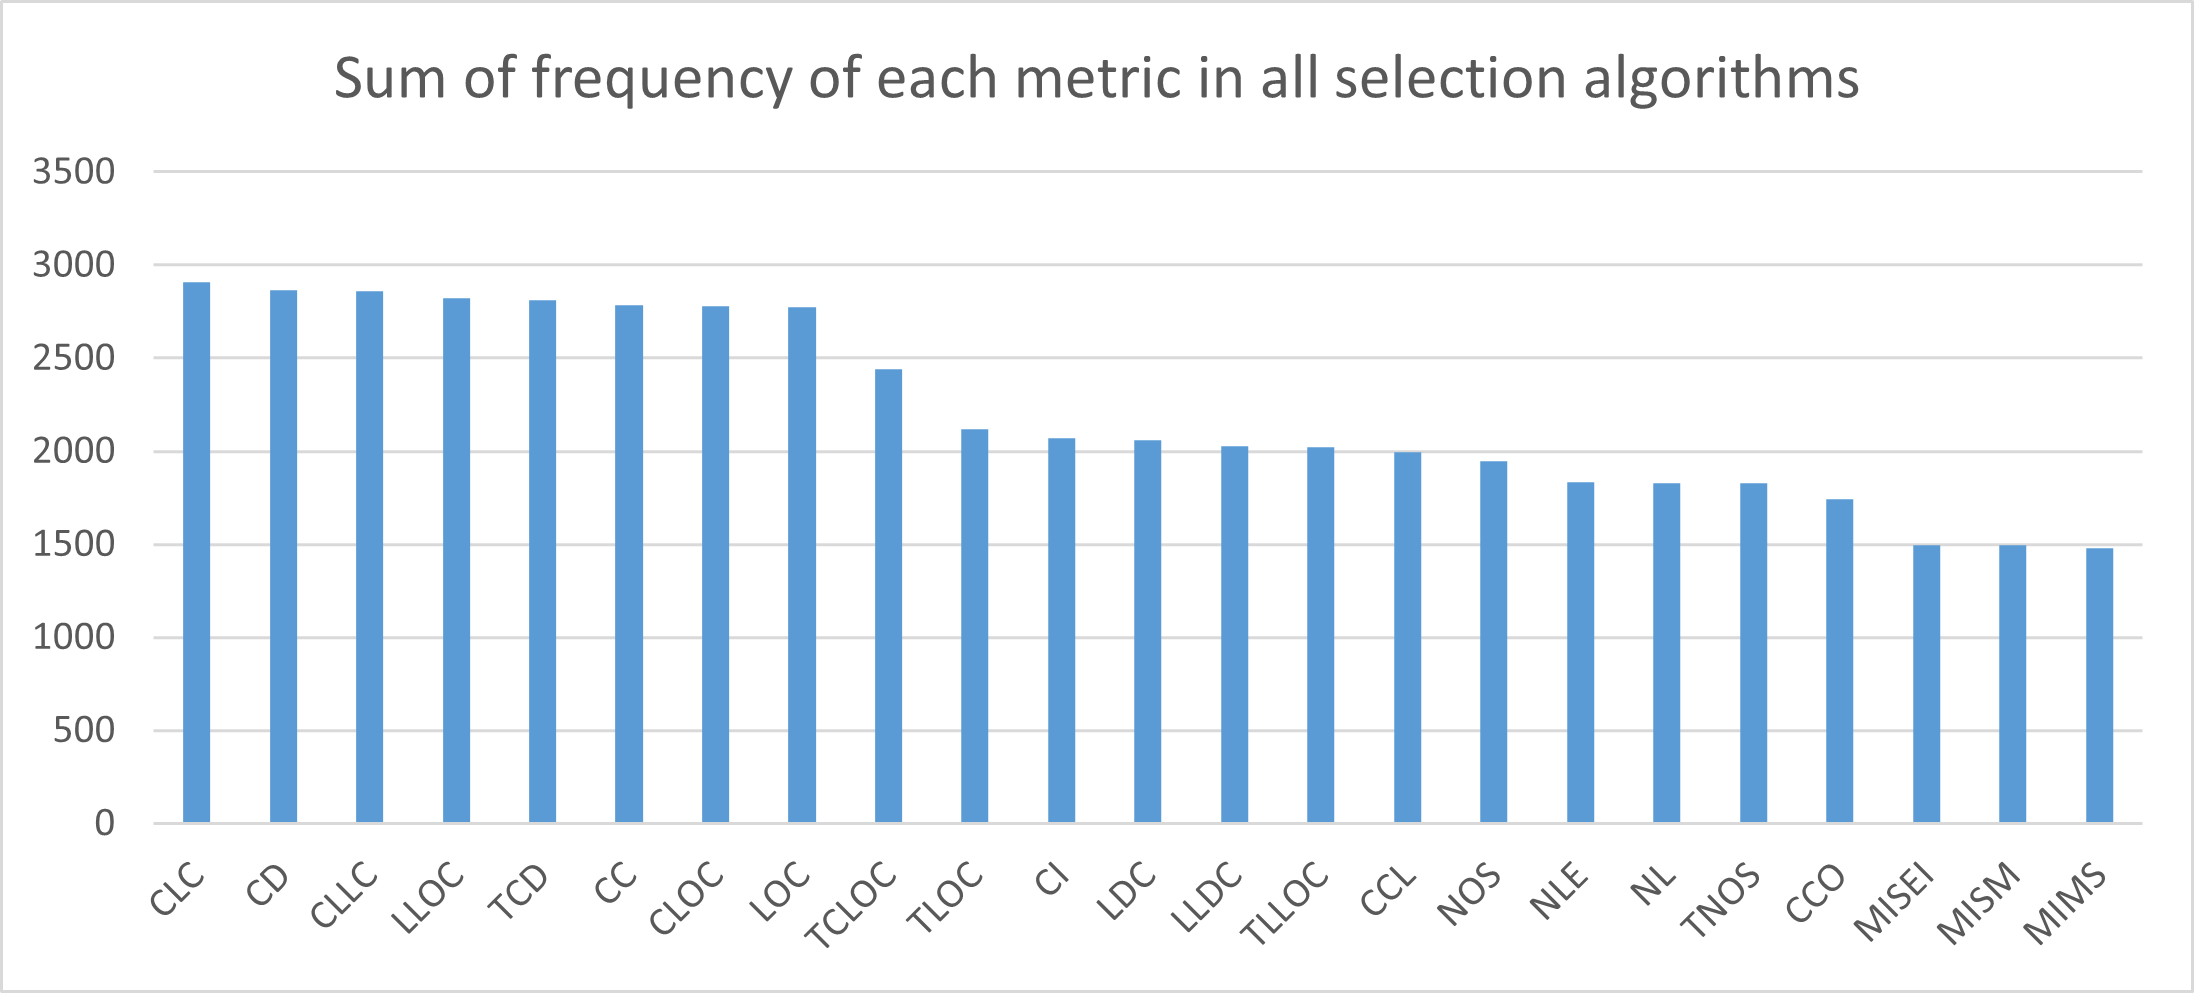
\includegraphics[scale=0.9]{chapters/chapter3/Sections/Research Questions/sections/RQ2/img/frec_all.png} %Change the figure name 
	\setstretch{1} %Interlineado 1
	\captionsetup{labelsep=period, labelfont=bf}
	\caption[Suma de la frecuencia de aparición de cada métrica en todos los algoritmos de selección]{Suma de la frecuencia de aparición de cada métrica en todos los algoritmos de selección} %[Se muestra en el índice]{Se muestra en el pie de figura}
	\label{fig:sum_frecuency}
\end{figure}


En la figura \ref{fig:frecuencyby}, se observa un patrón consistente: en promedio, los algoritmos de selección que incorporan el algoritmo de SU en su etapa de control de redundancia tienden a resultar en un menor número de características seleccionadas, en comparación con aquellos que utilizan la COS.

\begin{figure}[H]
	\centering
	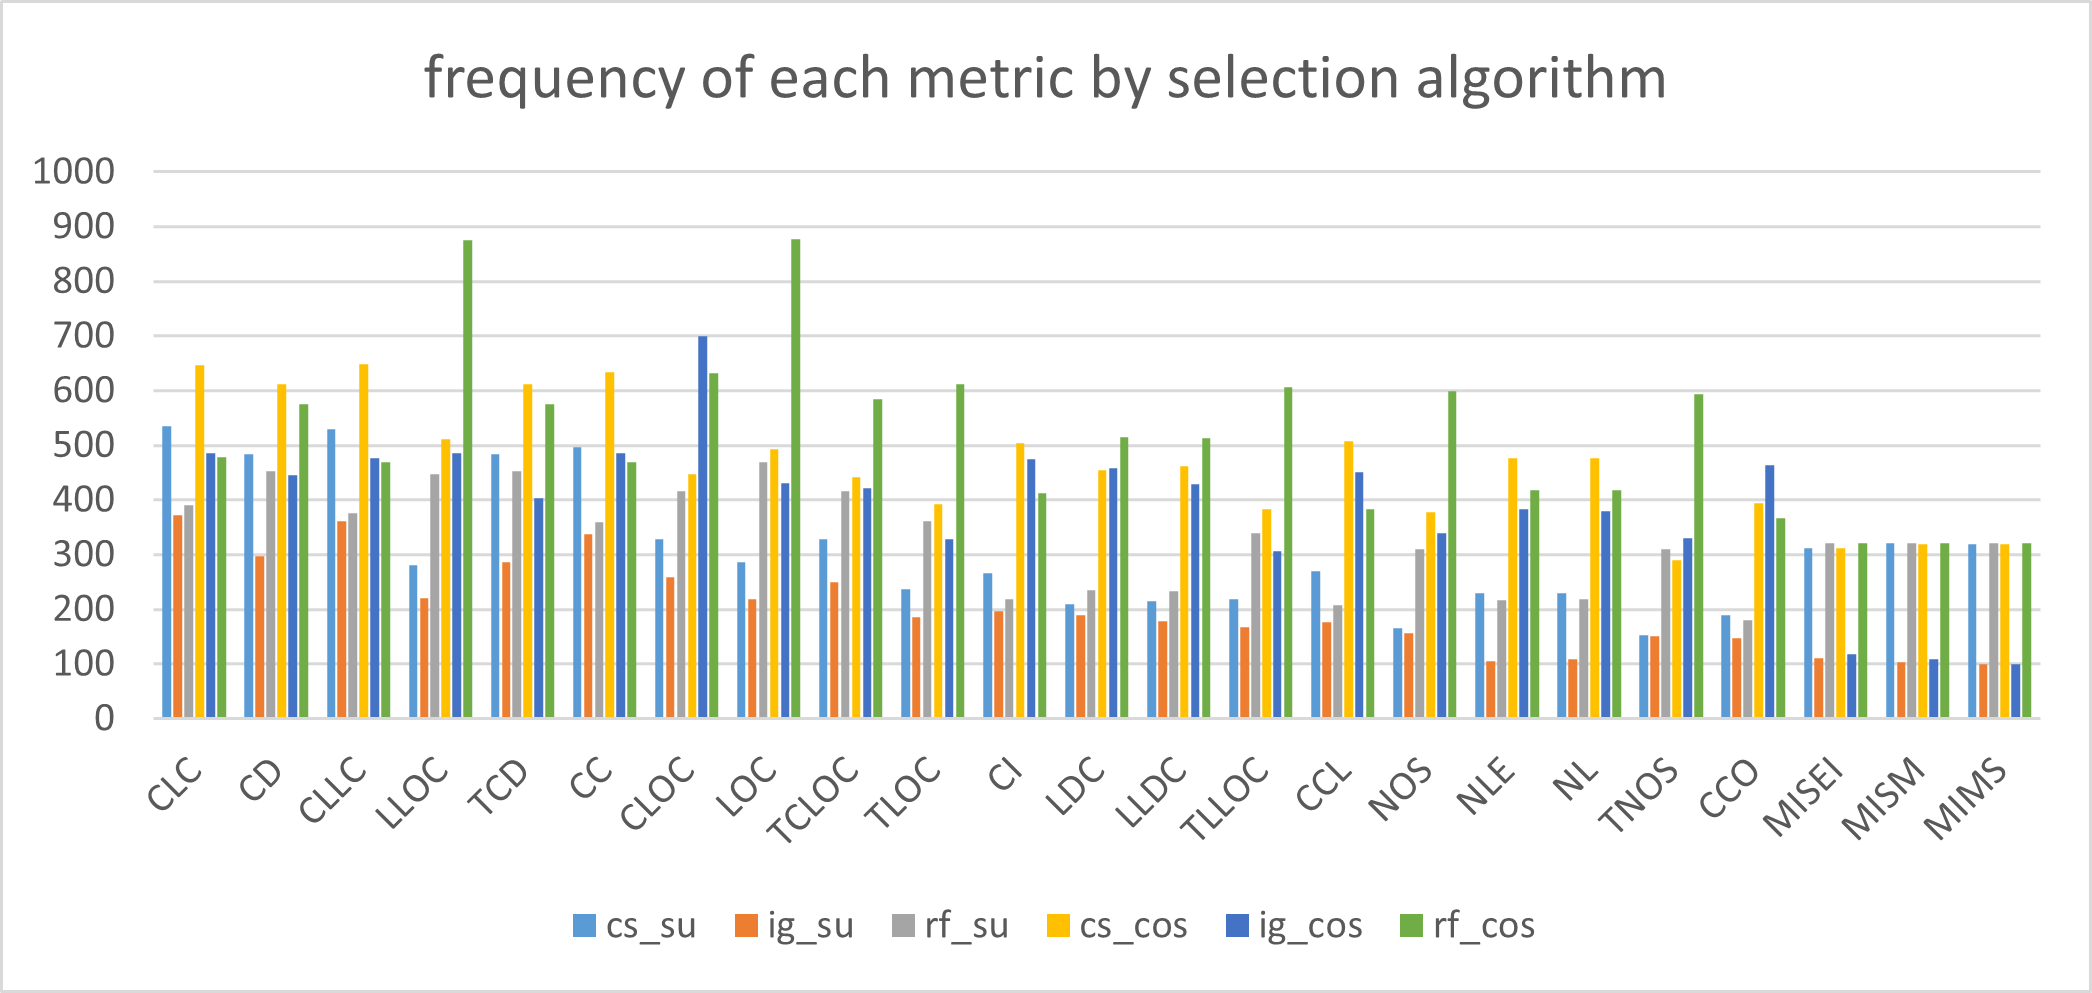
\includegraphics[scale=0.9]{chapters/chapter3/Sections/Research Questions/sections/RQ2/img/frec_by.png} %Change the figure name 
	\setstretch{1} %Interlineado 1
	\captionsetup{labelsep=period, labelfont=bf}
	\caption[Frecuencia de cada métrica \(\beta\) y algoritmo de selección]{Frecuencia de cada métrica \(\beta\) y algoritmo de selección}
 %[Se muestra en el índice]{Se muestra en el pie de figura}
	\label{fig:frecuencyby}
\end{figure}



En la la tabla \ref{table:selected_metrics} se muestra las métricas de código y la tabla \ref{table:cloneMetrics} separa las métricas de clone \cite{ferenc_automatically_2020} las cuales son calculadas a nivel de método y clase.

% Please add the following required packages to your document preamble:
% \usepackage{graphicx}
\begin{table}[H]
{
\fontsize{6pt}{6pt}\selectfont
\captionsetup{labelsep=period, labelfont=bf}
\caption{\label{table:selected_metrics} Ranking de las 15 mejores métricas de código seleccionadas}
\centering
\resizebox{\textwidth}{!}{%
\begin{tabular}{lllll}
\toprule
Abreviation & Full name                                   & Method & Class & File \\
\midrule
CD           & Comment Density                             & X      & X     &      \\
LLOC         & Logical Lines of Code                       & X      & X     & X    \\
TCD          & Total Comment Density                       & X      & X     &      \\
CLOC         & Comment Lines of Code                       & X      & X     & X    \\
LOC          & Lines of Code                               & X      & X     & X    \\
TCLOC        & Total Comment Lines of Code                 & X      & X     &      \\
TLOC         & Total Lines of Code                         & X      & X     &      \\
TLLOC        & Total Logical Lines of Code                 & X      & X     &      \\
NOS          & Number of Statements                        & X      & X     &      \\
NLE          & Nesting Level Else-If                       & X      & X     &      \\
NL           & Nesting Level                               & X      & X     &      \\
TNOS         & Total Number of Statements                  & X      & X     &      \\
MISEI        & Maintainability Index (SEI version)         & X      &       &      \\
MISM         & Maintainability Index (SourceMeter version) & X      &       &      \\
MIMS         & Maintainability Index (Microsoft version)   & X      &       &   \\
\bottomrule
\end{tabular}%
}
}

\end{table}

Como se evidencia en la Tabla \ref{table:selected_metrics}, las métricas seleccionadas prioritariamente corresponden al nivel de método, seguidas por las métricas a nivel de clase y, finalmente, las de archivo. Es importante destacar que la cantidad de métricas disponibles a nivel de archivo es considerablemente menor en comparación con las de nivel de método y clase. Paralelamente, según lo indicado en la Tabla \ref{metrics-table}, solo tres métricas - CLOC, LOC y LLOC - están presentes en los tres niveles mencionados. Estas métricas fueron seleccionadas entre las más contribuyentes a los modelos predictivos. Esto subraya la relevancia y eficacia de dichas métricas en la predicción de errores.

\begin{table}[h]
\centering{
\captionsetup{labelsep=period, labelfont=bf}
\caption{Best clone metrics selected}
\begin{tabular}{ll}
\toprule
Abreviatura & Nombre completo                        \\
\midrule
CLC          & Clone Line Coverage              \\
CLLC         & Clone Lines of Code              \\
CC           & Clone Coverage                   \\
CI           & Clone Instances                  \\
LDC          & Lines of Duplicated Code         \\
LLDC         & Logical Lines of Duplicated Code \\
CCL          & Clone Classes        \\
\bottomrule
\end{tabular}%


\label{table:cloneMetrics} 
}
\end{table}


En la tabla \ref{table:metric_cero_varia} se muestran las métricas que no tienen variación en sus datos, aquellas que contengan aproximadamente un 95\% o más de sus datos con un valor constante. 

 \begin{table}[H]
{
\fontsize{10pt}{10pt}\selectfont
\captionsetup{labelsep=period, labelfont=bf}
\caption{Características con poca variación en sus valores}
\label{table:metric_cero_varia}
\centering{
\begin{tabular}{llll}
\toprule
\textbf{Nombre   completo}          & \textbf{Valores} & \textbf{Cantidad} & \textbf{Total} \\
\midrule

WarningCritical                     & 0                & 159078            & 100\%          \\
\hline
Unnecessary and Unused   Code Rules & 0                & 159077            & 99.99\%        \\
                                    & 1                & 1                 & 0.01\%         \\
                                    \hline
Java Logging Rules                  & 0                & 159078            & 100\%          \\
\hline
Import Statement Rules              & 0                & 159007            & 99.95\%        \\
                                    & 1-5           & 71                & 0.15\%         \\
                                    \hline
Migration15 Rules                   & 0                & 150949            & 94.88\%        \\
                                    & 1-6,15           & 1171              & 0.73\%         \\
                                    \hline
WarningMinor                        & 0                & 159078            & 100\%          \\
\hline
Migration Rules                     & 0                & 159078            & 100\%          \\
\hline
Migration13 Rules                   & 0                & 159078            & 100\%          \\
\hline
Migration14 Rules                   & 0                & 159078            & 100\%          \\
\hline
MigratingToJUnit4 Rules             & 0                & 158991            & 99.94\%        \\
\hline
                                    & 1-4,6            & 87                & 0.06           \\
                                    \hline
JavaBean Rules                      & 0                & 159078            & 100\%          \\
\hline
Jakarta Commons Logging   Rules     & 0                & 155047            & 97.46\%        \\
                                    & 1-22           & 4039              & 2.54\%         \\
                                    \hline
JUnit Rules                         & 0                & 157826            & 99.21\%        \\
                                    & 01-9          & 1252              & 0.79\%         \\
                                    \hline
Finalizer Rules                     & 0                & 156912            & 98.63\%        \\
                                    & 1-81           & 2166              & 1.37\%         \\
                                    \hline
Empty Code Rules                    & 0                & 159054            & 99.98\%        \\
                                    & 1                & 24                & 0.02\%         \\
                                    \hline
Design Rules                        & 0                & 157537            & 99.03\%        \\
                                    & 1-15           & 1541              & 0.96\%         \\
                                    \hline
Comment Rules                       & 0                & 159078            & 100\%          \\
\hline
Clone Implementation Rules          & 0                & 159078            & 100\%          \\
\hline
Brace Rules                         & 0                & 159035            & 99.97\%        \\
\hline
                                    & 01-2           & 43                & 0.027\%        \\
                                    \hline
TNOS                                & 0                & 159077            & 99.99\%        \\
\hline
                                    & 1                & 1                 & 0.01          
\\\bottomrule
\end{tabular}
}
\captionsetup{labelsep=period, labelfont=bf}



}

\end{table}

De acuerdo con los análisis presentados en las tablas \ref{description-table} y \ref{table:metric_cero_varia}, se observa que, a excepción de la métrica TNOS, todas las demás métricas relacionadas con la violación de reglas presentan poca variación en sus datos (ver tabla \ref{table:smell_metrics}). Este patrón sugiere que dichas métricas podrían no ser particularmente relevantes para el proceso de predicción de errores en el contexto estudiado.

\textit{Advertencia sobre un posible artefacto de conteo.} Una explicación alternativa, no excluyente, para la alta frecuencia de selección de CLOC, LOC y LLOC es un artefacto de conteo: al ser las únicas tres métricas disponibles en los tres niveles de granularidad, tienen estructuralmente el triple de oportunidades de ser seleccionadas que una métrica exclusiva de un solo nivel, y el doble que una disponible en dos niveles. Los datos actuales no permiten distinguir, sin reprocesar los registros de selección normalizando por nivel de granularidad, entre valor predictivo genuino y este efecto de oportunidad; esta verificación se declara como trabajo futuro (Capítulo \ref{cap:conclusion}) y como amenaza a la validez de constructo (Capítulo \ref{cap:discusion}).

\noindent\fbox{%
\parbox{\dimexpr\textwidth-2\fboxsep-2\fboxrule\relax}{%
\textbf{Respuesta RQ2}
   Entre las métricas con mayor contribución se encuentran aquellas calculables en los tres niveles: método, clase y archivo, específicamente CLOC, LOC y LLOC, aunque parte de su preeminencia puede deberse a que tienen más oportunidades de ser seleccionadas. No obstante, según se detalla en la Tabla \ref{table:selected_metrics}, las métricas de código más relevantes para los modelos empleados en la selección de características son, en orden de importancia, aquellas a nivel de método, clase y archivo, respectivamente. En resumen, las métricas más relevantes para la predicción de errores son las métricas de código fuente, seguidas por las métricas de clonación de código, mientras que las métricas de violación de reglas (\textit{code smells}) quedan prácticamente fuera, con la excepción de TNOS.
}%
}
\vspace{12pt}
\section{Tercera pregunta de investigación}


\noindent\fbox{%
\parbox{\dimexpr\textwidth-2\fboxsep-2\fboxrule\relax}{%
\textbf{RQ3} ¿Como influye la variación de los parámetros de entrada a los algoritmos de análisis de relevancia y control de redundancia en los resultados de los modelos de clasificación?%
}%
}
\vspace{12pt}


\section{Estadísticas Descriptivas de FMeasure}

Las estadísticas descriptivas de la columna \textbf{FMeasure} son las siguientes:

\begin{itemize}
    \item Cantidad de registros (count): 13,916
    \item Media (mean): 0.547
    \item Desviación estándar (std): 0.104
    \item Valor mínimo (min): 0.274
    \item Percentil 25\%: 0.488
    \item Mediana (50\%): 0.529
    \item Percentil 75\%: 0.610
    \item Valor máximo (max): 0.844
\end{itemize}

Estos datos nos indican que la media de la medida F es aproximadamente 0.547, con una variabilidad moderada (desviación estándar de 0.104). El rango de los valores de FMeasure va desde 0.274 hasta 0.844.

\section{Correlación entre FMeasure, Rank y \(\beta\)}

A continuación, examinaré la correlación entre las columnas FMeasure, Rank y \(\beta\) para entender cómo se relacionan estas variables entre sí. Posteriormente, representaré visualmente estas relaciones.

\begin{figure}[H]
    \centering
    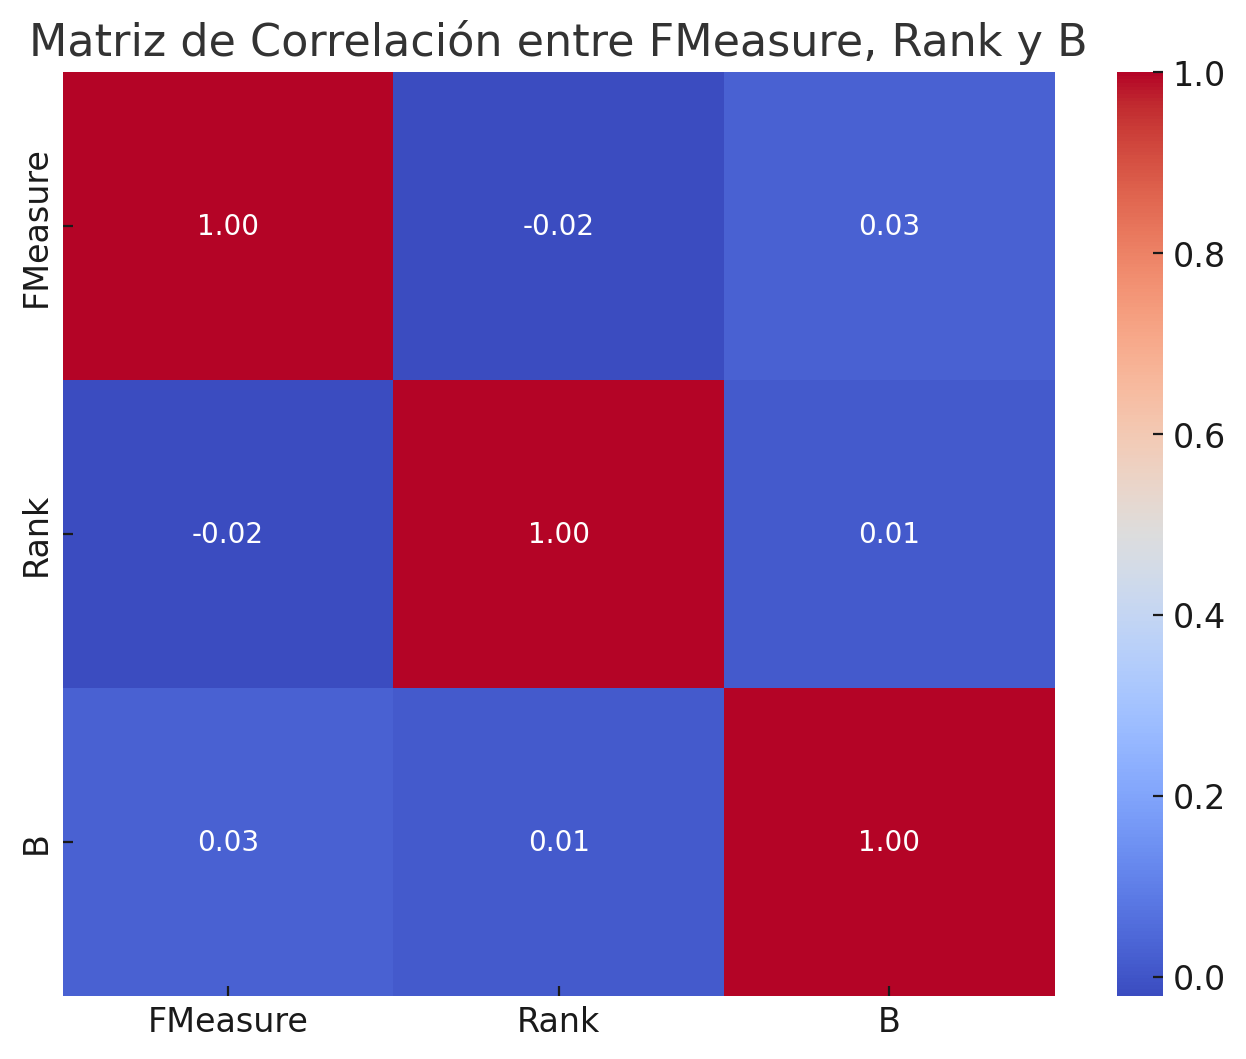
\includegraphics[width=100mm, height=80mm,]{chapters/chapter3/Sections/Research Questions/sections/RQ3/img/matriz.png}
    \setstretch{1} %Interlineado 1
	\captionsetup{labelsep=period, labelfont=bf}
    \caption{Frecuencia de cada métrica \(\beta\) y algoritmo de selección}
    \label{fig:frecuencyby}
\end{figure}

La matriz de correlación entre \textbf{FMeasure}, \textbf{Rank} y \textbf{B} revela lo siguiente:
{
\fontsize{14pt}{14pt}\selectfont
\begin{itemize}
    \item{Correlación entre FMeasure y Rank:} -0.021, lo que indica una correlación negativa muy débil. 
    \item{Correlación entre FMeasure y  \(\beta\):} 0.027, sugiriendo una correlación positiva muy débil. 
    \item{Correlación entre Rank y \(\beta\):} 0.011, lo que implica una correlación positiva casi inexistente.
\end{itemize}
}

Estas correlaciones sugieren que ni \textit{Rank} ni \textit{B} tienen una relación fuerte con \textit{FMeasure}.

Aunque no se observa una correlación fuerte entre los parámetros de entrada y el FMeasure, la Figura \ref{fig:FMeasure_rank_b} ilustra que, generalmente, valores menores de 'Rank' y mayores de 'B' se asocian con mejores resultados de FMeasure. Además, se identifica una tendencia descendente en los valores de FMeasure a medida que aumenta el 'Rank' para los tres valores distintos de 'B' evaluados.

\begin{figure}[H]
    \centering
    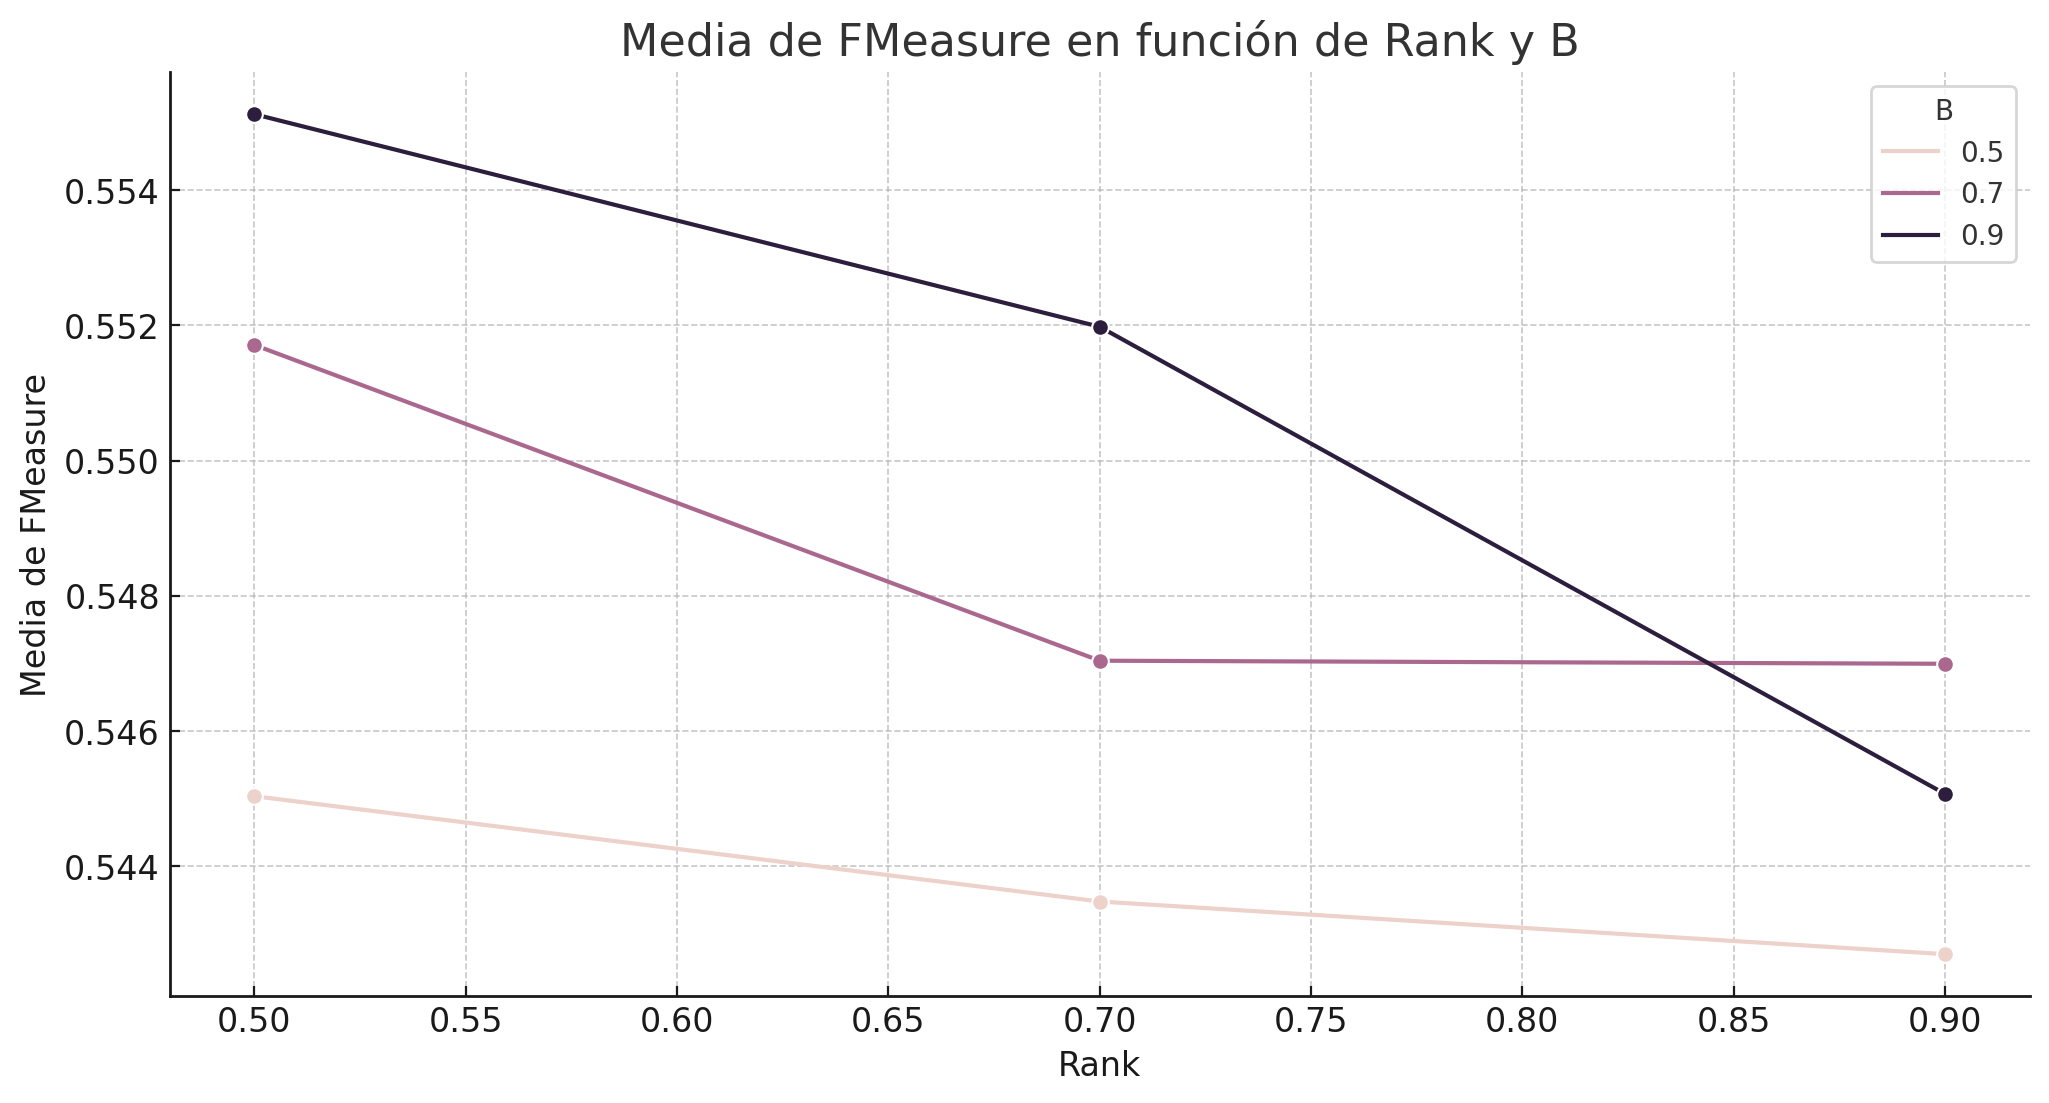
\includegraphics[width=150mm, height=120mm,]{chapters/chapter3/Sections/Research Questions/sections/RQ3/img/medida f en funcion de ran y b.png}
     \setstretch{1} %Interlineado 1
	\captionsetup{labelsep=period, labelfont=bf}
    \caption{Medición basada en rango y $\beta$}
    \label{fig:FMeasure_rank_b}
\end{figure}

En las tablas \ref{table:b_u_c_m}, \ref{table:b_u_c_c} y \ref{table:b_u_c_f} observamos que se obtienen valores similares a los obtenidos en la linea base (\ref{table:original_result_average}) pero con una disminución significativa de las características ingresadas en los modelos de clasificación. 

\noindent\fbox{%
\parbox{\dimexpr\textwidth-2\fboxsep-2\fboxrule\relax}{%
\textbf{Respuesta RQ3} 
En resumen, se observa que los parámetros de entrada utilizados en los algoritmos de análisis de relevancia y control de redundancia no presentan una correlación fuerte con el FMeasure. Sin embargo, se identifica que valores menores de 'Rank' y mayores de \( \beta \)  se asocian, en promedio, con mejores resultados de FMeasure. Paralelamente, se destaca que los algoritmos de selección reducen la cantidad de características ingresadas a los algoritmos, manteniendo o incluso mejorando los valores de FMeasure. Esto sugiere que, a pesar de la diversidad de los resultados, los valores seleccionados fueron eficaces para cumplir su propósito con un conjunto reducido de características.
}%
}
\vspace{12pt}
\section{Cuarta pregunta de investigación}
\label{sec:RQ4}

\noindent\fbox{%
\parbox{\dimexpr\textwidth-2\fboxsep-2\fboxrule\relax}{%
\textbf{RQ4} ¿Cómo influyen los algoritmos de balanceo de clases ROS, RUS y SMOTE en los resultados de los clasificadores?%
}%
}
\vspace{12pt}

\subsection{Desbalance de BugHunter}

La Tabla \ref{table:count_bug_nobug} muestra el número de instancias con error (\textit{bug}) y sin error por proyecto y nivel. En la mayoría de los proyectos predominan las instancias sin error, aunque la proporción varía considerablemente entre proyectos y niveles.

% Please add the following required packages to your document preamble:
% \usepackage{graphicx}
\begin{table}[H]
\captionsetup{labelsep=period, labelfont=bf}
\caption{\label{table:count_bug_nobug} Resumen de desequilibrio por nivel}
\centering
\resizebox{\textwidth}{!}{%
\begin{tabular}{lllllll}
\toprule
                               & \multicolumn{2}{c}{Método} & \multicolumn{2}{c}{Clase} & \multicolumn{2}{c}{Archivo} \\
                               \midrule
Proyecto                        & Bug       & Sin bug    & Bug      & Sin bug    & Bug      & Sin bug   \\
\midrule
oryx                           & 100       & 756            & 81       & 565            & 80       & 528           \\
antlr4                         & 132       & 768            & 132      & 230            & 156      & 223           \\
BroadleafCommerce              & 1337      & 3996           & 1569     & 1672           & 1733     & 1828          \\
mct                            & 26        & 81             & 21       & 51             & 15       & 43            \\
junit                          & 112       & 400            & 112      & 226            & 96       & 107           \\
netty                          & 3620      & 9923           & 2618     & 3973           & 2178     & 2947          \\
ceylon-ide-eclipse             & 660       & 1731           & 520      & 957            & 417      & 747           \\
titan                          & 287       & 736            & 195      & 311            & 199      & 287           \\
all                            & 58810     & 100268         & 41087    & 43475          & 35507    & 34581         \\
elasticsearch                  & 19784     & 31746          & 15769    & 15875          & 13068    & 12052         \\
mcMMO                          & 503       & 865            & 357      & 511            & 369      & 511           \\
orientdb                       & 4465      & 8732           & 2153     & 2617           & 2107     & 2341          \\
neo4j                          & 3175      & 6523           & 2068     & 2601           & 1824     & 2120          \\
hazelcast                      & 23830     & 32617          & 14926    & 13259          & 12881    & 10472         \\
MapDB                          & 644       & 1140           & 487      & 522            & 311      & 277           \\
Android-Universal-Image-Loader & 135       & 254            & 79       & 105            & 73       & 98        \\
\bottomrule
\end{tabular}%
}

\end{table}

La Tabla \ref{tab:desbalance} resume esta distribución tras binarizar el atributo \textit{Number of Bugs}. El desequilibrio de BugHunter es moderado si se compara con los conjuntos clásicos de PFS ---como NASA o PROMISE, donde la clase con error suele representar menos del 10\,\% de las instancias \cite{8494821}---: la mediana de instancias \textit{bug} entre los 15 proyectos es del 28,1\,\% a nivel de método, 41,1\,\% a nivel de clase y 42,7\,\% a nivel de archivo, y en tres proyectos (\textit{hazelcast}, \textit{MapDB} y \textit{elasticsearch}) la clase \textit{bug} llega a ser mayoritaria a nivel de archivo. Esta característica es consecuencia directa del diseño de BugHunter, que solo incluye elementos de código efectivamente afectados por errores. El caso más desequilibrado es \textit{oryx} (razón no-bug:bug de 7,6:1 a nivel de método), lo que debe tenerse presente al interpretar su desempeño, el más alto del estudio.

\begin{table}[H]
\centering
\caption{Proporción de instancias con error (\textit{bug}) por nivel de granularidad, sobre los 15 proyectos individuales}
\label{tab:desbalance}
\resizebox{\textwidth}{!}{%
\begin{tabular}{lccccc}
\toprule
Nivel & Mediana & Mín. (proyecto) & Máx. (proyecto) & ``All'' & Razón mediana \\
      & \% bug  &                 &                 & \% bug  & no-bug:bug \\
\midrule
Método  & 28,1 & 11,7 (\textit{oryx}) & 42,2 (\textit{hazelcast}) & 37,0 & 2,6:1 \\
Clase   & 41,1 & 12,5 (\textit{oryx}) & 53,0 (\textit{hazelcast}) & 48,6 & 1,4:1 \\
Archivo & 42,7 & 13,2 (\textit{oryx}) & 55,2 (\textit{hazelcast}) & 50,7 & 1,3:1 \\
\bottomrule
\end{tabular}}
\end{table}

\subsection{Efecto del balanceo sobre el \textit{F-measure} ponderado}

La Tabla \ref{tab:balance} resume el \textit{F-measure} promedio de las 13.916 ejecuciones agrupadas por técnica de balanceo, comparando el conjunto de entrenamiento original con su versión balanceada (el conjunto de prueba nunca se balancea). Con las tres técnicas, balancear el conjunto de entrenamiento no mejoró el \textit{F-measure} promedio respecto a entrenar con la distribución original. El efecto fue más marcado en RUS, cuya eliminación de instancias de la clase mayoritaria redujo la información disponible para el entrenamiento. Las desviaciones estándar fueron similares entre ambas condiciones (0,108 sin balancear; 0,104, 0,082 y 0,105 balanceando con ROS, RUS y SMOTE, respectivamente).

\begin{table}[H]
\centering
\caption{\textit{F-measure} promedio según técnica de balanceo (13.916 ejecuciones)}
\label{tab:balance}
\begin{tabular}{lccc}
\toprule
Técnica & Sin balancear & Balanceado & $\Delta$ \\
\midrule
ROS   & 0,555 & 0,548 & $-0{,}007$ \\
RUS   & 0,555 & 0,524 & $-0{,}031$ \\
SMOTE & 0,555 & 0,548 & $-0{,}007$ \\
\bottomrule
\end{tabular}
\end{table}

\begin{figure}[H]
    \centering
    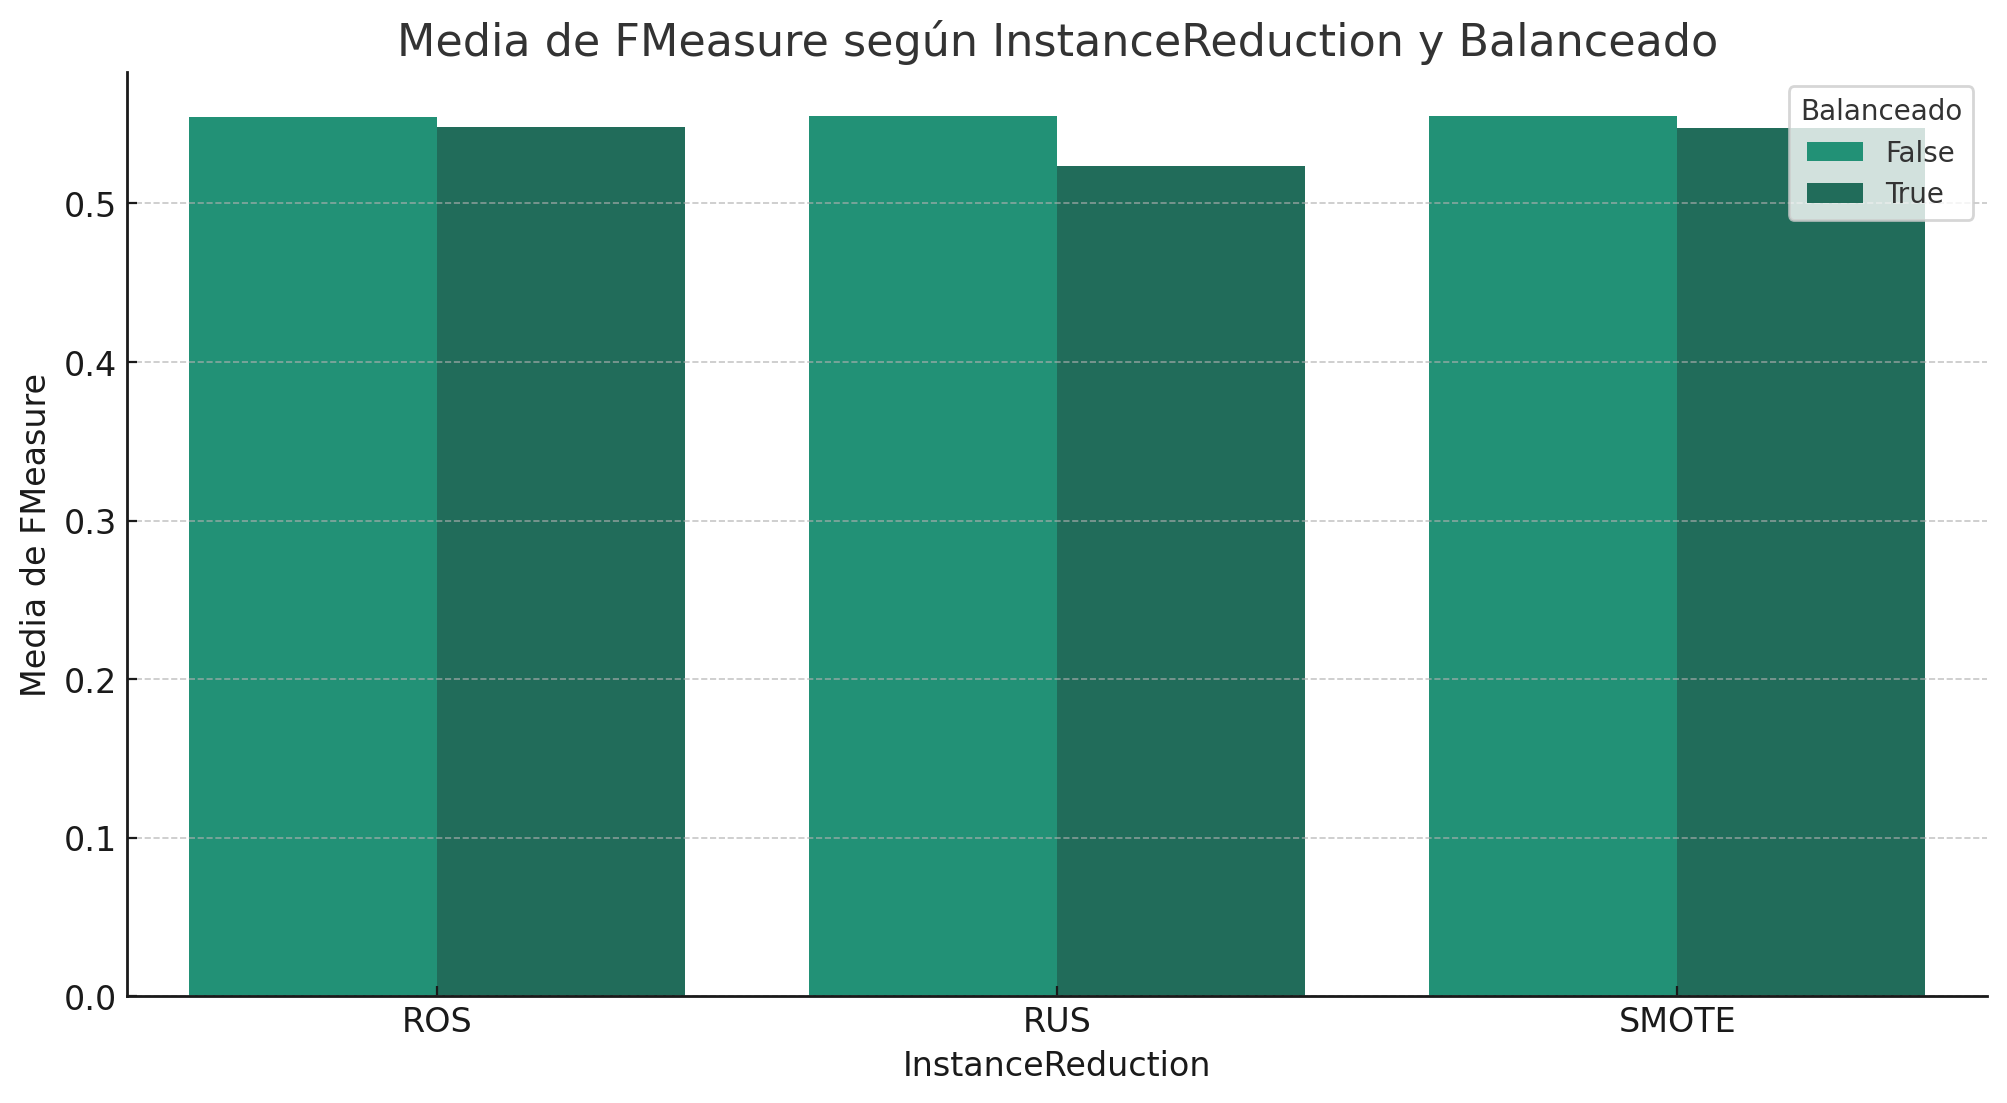
\includegraphics[width=150mm, height=120mm,]{chapters/chapter3/Sections/Research Questions/sections/RQ4/img/InstancereductionBalanceado.png}
     \setstretch{1} %Interlineado 1
	\captionsetup{labelsep=period, labelfont=bf}
    \caption{\textit{F-measure} medio según algoritmo de balanceo y condición de balanceo del entrenamiento}
    \label{fig:ROSRUSSMOTE}
\end{figure}

Para contrastar formalmente esta observación se aplicó una prueba de Wilcoxon de rangos con signo \cite{wilcoxon1945}, pareada por conjunto de datos, sobre el mejor \textit{F-measure} balanceado frente al mejor sin balancear de cada uno de los 16 conjuntos por nivel, complementada con el tamaño de efecto $\delta$ de Cliff \cite{cliff1993}. A nivel de método la diferencia resultó estadísticamente significativa a favor de la versión sin balancear ($p = 0{,}012$), aunque con un tamaño de efecto insignificante ($\delta = 0{,}07$); a nivel de clase ($p = 0{,}48$) y de archivo ($p = 0{,}86$) no se detectaron diferencias significativas, y al agrupar los tres niveles el resultado quedó en el límite de la significancia ($p = 0{,}052$). En los cuatro casos el tamaño de efecto fue insignificante ($|\delta| < 0{,}15$).

\subsection{Efecto del balanceo sobre la clase minoritaria}

Estas cifras deben interpretarse con cautela. Las medias de la Tabla \ref{tab:balance} se analizaron de forma descriptiva sobre todas las ejecuciones, mientras que la prueba estadística se aplicó a la mejor configuración por proyecto, sujeta a un sesgo de selección optimista. Además, el \textit{F-measure} agregado pondera ambas clases por su frecuencia, de modo que la contribución de la clase de interés práctico (\textit{bug}) queda diluida. Este efecto está acotado por el desequilibrio moderado de BugHunter (Tabla \ref{tab:desbalance}), pero no desaparece: la línea base del conjunto ``All'' a nivel de método (Tabla \ref{tab:porclase}) muestra que un \textit{F-measure} ponderado de 0,565 convive con un \textit{F-measure} de 0,356 para la clase \textit{bug} y un MCC cercano a cero.

Dos fuentes de evidencia permiten ir más allá de la métrica agregada. La primera son las matrices de confusión que Weka entrega para las mejores configuraciones a nivel de método (Tabla \ref{table:weka_method_smote_b}), a partir de las cuales se calculan el \textit{F-measure} de la clase \textit{bug} y el MCC (Sección \ref{sec:validacion_flujos}). Sobre los 16 conjuntos, entrenar con SMOTE reduce la mediana del \textit{F-measure} ponderado de 0,600 a 0,581, pero eleva la mediana del \textit{F-measure} de la clase \textit{bug} de 0,280 a 0,334; en MCC, en cambio, la diferencia es pequeña y de signo opuesto (0,070 frente a 0,056). Debe notarse que estas configuraciones fueron elegidas por su \textit{F-measure} ponderado y no por su desempeño en la clase minoritaria. La segunda fuente, más completa, es el análisis de sensibilidad (Sección \ref{sec:sensibilidad}), que almacena las métricas por clase para sus 28.440 ejecuciones y muestra que el balanceo mejora de forma consistente el \textit{F-measure} de la clase \textit{bug} y el MCC en los tres clasificadores evaluados, aun cuando el \textit{F-measure} ponderado apenas varía.

\subsection{¿Qué técnica de balanceo es más efectiva?}

La respuesta depende del objetivo. La Tabla \ref{tab:balanceo_tecnica} resume, sobre las ejecuciones del análisis de sensibilidad en los 15 proyectos individuales, la mediana de cada métrica según la técnica de balanceo. Con \textit{Random Forest} y XGBoost, RUS obtiene el mayor \textit{F-measure} de la clase \textit{bug} y el mejor MCC, pero también el menor \textit{F-measure} ponderado: al eliminar instancias de la clase mayoritaria, el modelo predice defectos con más frecuencia, lo que mejora su detección a costa de más falsos positivos. ROS y SMOTE ofrecen un compromiso intermedio, con mejoras más moderadas en la clase \textit{bug} y una pérdida menor en el agregado. Con la SVM lineal, las tres técnicas producen mejoras similares y grandes en la clase \textit{bug}, porque sin balanceo este clasificador casi no predice defectos. Por tanto, si el objetivo es detectar la mayor cantidad posible de código defectuoso, RUS es la técnica más efectiva; si se busca preservar el desempeño global, ROS o SMOTE son preferibles.

\begin{table}[H]
\centering
\caption{Mediana del desempeño por técnica de balanceo en el análisis de sensibilidad (15 proyectos individuales, todas las configuraciones)}
\label{tab:balanceo_tecnica}
\begin{tabular}{llccc}
\toprule
Clasificador & Balanceo & \textit{F-measure} ponderado & \textit{F-measure} bug & MCC \\
\midrule
RF   & Ninguno & 0,537 & 0,325 & $-0{,}015$ \\
RF   & ROS     & 0,529 & 0,356 & $-0{,}008$ \\
RF   & RUS     & 0,513 & 0,417 & 0,009 \\
RF   & SMOTE   & 0,532 & 0,343 & $-0{,}013$ \\
\midrule
XGB  & Ninguno & 0,540 & 0,318 & 0,003 \\
XGB  & ROS     & 0,537 & 0,367 & 0,001 \\
XGB  & RUS     & 0,524 & 0,427 & 0,027 \\
XGB  & SMOTE   & 0,542 & 0,346 & $-0{,}004$ \\
\midrule
SVM  & Ninguno & 0,551 & 0,171 & 0,038 \\
SVM  & ROS     & 0,562 & 0,423 & 0,086 \\
SVM  & RUS     & 0,558 & 0,426 & 0,081 \\
SVM  & SMOTE   & 0,565 & 0,425 & 0,087 \\
\bottomrule
\end{tabular}
\end{table}

Las medianas de MCC cercanas a cero reflejan que la tabla incluye todas las configuraciones de selección, también las peores; las mejoras sobre la mejor configuración de cada proyecto se presentan en la Tabla \ref{tab:sensibilidad}.

\noindent\fbox{%
\parbox{\dimexpr\textwidth-2\fboxsep-2\fboxrule\relax}{%
\textbf{Respuesta RQ4}
Balancear solo el conjunto de entrenamiento con ROS, RUS o SMOTE no mejora el \textit{F-measure} ponderado cuando el conjunto de prueba conserva la distribución real de clases; RUS lo empeora de forma más marcada ($-0{,}031$). La diferencia entre las mejores configuraciones con y sin balanceo tiene un tamaño de efecto insignificante ($|\delta| < 0{,}15$) en los tres niveles. Sin embargo, el balanceo sí desplaza el desempeño hacia la clase de interés práctico: aumenta el \textit{F-measure} de la clase \textit{bug} y, en el análisis de sensibilidad, también el MCC. La conclusión de RQ4 depende, por tanto, de la métrica de evaluación empleada. Entre las técnicas, RUS maximiza la detección de defectos y ROS y SMOTE preservan mejor el desempeño global.
}%
}
\vspace{12pt}

\section{Quinta pregunta de investigación}

Nuestra ultima pregunta de investigación va enfocada a diferenciar los resultados entre el conjunto de datos resumen (unión de todos los proyectos en cada nivel) y los resultados individuales por proyecto.

\noindent\fbox{%
\parbox{\dimexpr\textwidth-2\fboxsep-2\fboxrule\relax}{%
\textbf{RQ5} ¿Que diferencias existen entre el proyecto resumen y los proyectos individuales en los resultados obtenidos en las preguntas anteriores?%
}%
}
\vspace{12pt}

El conjunto de datos All esta diseñado a partir de la unión de todos los conjuntos de datos en el mismo nivel de los 15 proyectos seleccionados, por ende existe un conjunto All para cada nivel método, clase y archivo. Contiene una mayor cantidad de registros que todos los proyectos individuales por su origen como se puede observar en la tabla \ref{table:count_bug_nobug}.

Iniciando con el análisis de los resultados base obtenidos en la sección \ref{sec:datasetoriginal}, observamos en las tablas \ref{table:original_result_weka_method_result}, \ref{table:original_result_weka_class_result} y \ref{table:original_result_weka_file_result} que en ninguno de los 3 niveles se obtienen los mejores resultados de F-measure para el proyecto All, pero tampoco siendo los peores.

\begin{table}[H]
\captionsetup{labelsep=period, labelfont=bf}
\caption{\label{table:min_max_all} Resultados base enfocados al proyecto ``All''}
\centering
\begin{tabular}{llll}
\toprule
Project & METHOD & CLASS & FILE  \\\midrule

Best    & 0,852  & 0,787 & 0,77  \\
All     & 0,579  & 0,484 & 0,482 \\
Min     & 0,486  & 0,338 & 0,344 \\
\bottomrule
\end{tabular}

 

\end{table}

Este escenario se observa consistentemente en respuesta a la pregunta de investigación RQ1 (véase Sección \ref{sec:RQ1}), como se ilustra en las Tablas \ref{table:b_u_c_m}, \ref{table:b_u_c_c}, y \ref{table:b_u_c_f}. A pesar de implementar la selección de características y el balanceo de clases, los resultados no alcanzan un nivel óptimo de rendimiento. Este fenómeno sugiere que la amalgama de métricas de código procedentes de diversos proyectos, los cuales pueden variar significativamente en metodologías de desarrollo, equipos de programación y objetivos, no contribuye necesariamente a la mejora de la precisión de los clasificadores. Se infiere que un análisis a nivel de proyecto individual es más fructífero, ya que los errores detectados en cada proyecto podrían estar intrínsecamente relacionados con aspectos específicos de desarrollo y estructura propios del software en cuestión. Por consiguiente, la expansión del volumen de datos mediante la combinación de métricas de diferentes proyectos no garantiza una mejora en los resultados, según se desprende de nuestro análisis.

\noindent\fbox{%
\parbox{\dimexpr\textwidth-2\fboxsep-2\fboxrule\relax}{%
\textbf{Respuesta RQ5} 
 El proyecto resumen cuenta con una mayor cantidad de registros unificando los diferentes proyectos, pero aun así esto no conlleva a la mejora de los resultados de los clasificadores en ninguna de los escenarios analizados: conjunto de datos original, selección de características y balanceo de clases. Por tanto, concluimos que se obtienen mejores resultados entrenando los clasificadores con métricas de software individuales, dado que cada software tiene sus aspectos específicos de desarrollo 
}%
}
\vspace{12pt}

\section{Validación cruzada entre herramientas: Weka y \textit{scikit-learn}}
\label{sec:validacion_flujos}

El estudio principal combina dos herramientas: la selección de características, la partición estratificada 67/33 y el balanceo del entrenamiento se realizan en Python, mientras que la clasificación con \textit{Random Forest} se ejecuta en Weka en modalidad \textit{Supplied test set} (Sección \ref{sec:RQ1}). El análisis de sensibilidad (Sección \ref{sec:sensibilidad}), en cambio, se ejecuta completamente en \textit{scikit-learn}. Para verificar que ambos flujos son intercambiables, se compararon las 32 mejores configuraciones a nivel de método registradas en Weka ---16 conjuntos, sin balancear y con SMOTE (Tabla \ref{table:weka_method_smote_b})--- con la configuración idéntica (proyecto, esquema, \textit{Rank}, $\beta$ y balanceo) del análisis de sensibilidad ejecutado con \textit{Random Forest} en \textit{scikit-learn}. La comparación no requiere reejecutar modelos y se implementó en el \textit{script} \texttt{validar\_weka\_vs\_sklearn.py}.

\begin{table}[H]
\caption{\label{table:weka_method_smote_b}Mejor resultado por proyecto a nivel de método en Weka (\textit{Supplied test set}), sin balancear y balanceando el entrenamiento con SMOTE, con su matriz de confusión (clase positiva: \textit{bug})}
\resizebox{\textwidth}{!}{
\begin{tabular}{lllllllllllll}
\hline
\multicolumn{13}{c}{\textbf{SMOTE}}                                                                                                                                                                               \\\hline 
\multicolumn{13}{c}{\textbf{MÉTODO}}                                                                                                                                                                       \\\hline
\textbf{Proyecto}               & \textbf{Precisión} & \textbf{Recall} & \textbf{F-measure} & \textbf{Variación} & \textbf{Rank} & \textbf{$\beta$} & \textbf{Esquema} & \textbf{TP} & \textbf{TN} & \textbf{FN} & \textbf{FP} & \textbf{Balanceado} \\\hline
oryx                           & 0,825              & 0,859           & 0,838             & 0,029              & 0.7           & 0.7        & CS\_SU                  & 5           & 238         & 28          & 12          & No               \\
                           & 0,82               & 0,799           & 0,809             &                    & 0.7           & 0.7        & CS\_SU                  & 9           & 217         & 24          & 33          & Sí                \\
antlr4                         & 0,8                & 0,795           & 0,797             & 0,026              & 0.5           & 0.9        & RF\_COS                 & 15          & 221         & 29          & 32          & Sí                \\
                         & 0,746              & 0,801           & 0,771             &                    & 0.5           & 0.9        & RF\_COS                 & 3           & 235         & 41          & 18          & No               \\
BroadleafCommerce              & 0,757              & 0,77            & 0,762             & 0                  & 0.5           & 0.5        & CS\_COS                 & 196         & 1160        & 245         & 159         & Sí                \\
              & 0,76               & 0,78            & 0,762             &                    & 0.5           & 0.5        & CS\_COS                 & 169         & 1203        & 272         & 116         & No               \\
mct                            & 0,706              & 0,694           & 0,7               & 0,016              & 0.7           & 0.7        & IG\_SU                  & 4           & 21          & 5           & 6           & No               \\
                            & 0,716              & 0,667           & 0,684             &                    & 0.7           & 0.7        & IG\_SU                  & 5           & 19          & 4           & 8           & Sí                \\
junit                          & 0,676              & 0,722           & 0,694             & 0,02               & 0.9           & 0.9        & IG\_COS                 & 6           & 116         & 31          & 16          & No               \\
                          & 0,668              & 0,68            & 0,674             &                    & 0.9           & 0.9        & IG\_COS                 & 8           & 107         & 29          & 25          & Sí                \\
netty                          & 0,638              & 0,684           & 0,653             & 0,013              & 0.9           & 0.9        & RF\_COS                 & 234         & 2823        & 961         & 452         & No               \\
                          & 0,63               & 0,654           & 0,64              &                    & 0.9           & 0.9        & RF\_COS                 & 298         & 2624        & 897         & 651         & Sí                \\
titan                          & 0,634              & 0,663           & 0,645             & 0,052              & 0.7           & 0.7        & CS\_SU                  & 25          & 199         & 70          & 44          & No               \\
                          & 0,607              & 0,583           & 0,593             &                    & 0.7           & 0.7        & CS\_SU                  & 34          & 163         & 61          & 80          & Sí                \\
ceylon-ide-eclipse             & 0,601              & 0,657           & 0,62              & 0,008              & 0.7           & 0.7        & IG\_COS                 & 33          & 486         & 185         & 86          & No               \\
             & 0,6                & 0,629           & 0,612             &                    & 0.7           & 0.7        & IG\_COS                 & 46          & 451         & 172         & 121         & Sí                \\
mcMMO                          & 0,577              & 0,604           & 0,581             & 0,016              & 0.7           & 0.9        & IG\_COS                 & 48          & 225         & 118         & 61          & No               \\
                          & 0,561              & 0,569           & 0,565             &                    & 0.7           & 0.9        & IG\_COS                 & 62          & 195         & 104         & 91          & Sí                \\
all                            & 0,567              & 0,59            & 0,573             & 0,004              & 0.9           & 0.9        & RF\_COS                 & 5958        & 25034       & 13449       & 8055        & No               \\
                            & 0,563              & 0,579           & 0,569             &                    & 0.9           & 0.9        & RF\_COS                 & 6610        & 23775       & 12797       & 9314        & Sí                \\
elasticsearch                  & 0,567              & 0,586           & 0,571             & 0,014              & 0.5           & 0.9        & CS\_COS                 & 2189        & 7768        & 4340        & 2708        & No               \\
                  & 0,555              & 0,559           & 0,557             &                    & 0.5           & 0.9        & CS\_COS                 & 2593        & 6920        & 3936        & 3556        & Sí                \\
orientdb                       & 0,557              & 0,598           & 0,569             & 0,017              & 0.7           & 0.5        & RF\_COS                 & 320         & 2284        & 1154        & 598         & No               \\
                       & 0,551              & 0,553           & 0,552             &                    & 0.7           & 0.5        & RF\_COS                 & 492         & 1915        & 982         & 967         & Sí                \\
hazelcast                      & 0,551              & 0,559           & 0,553             & 0,003              & 0.7           & 0.7        & CS\_COS                 & 3206        & 7202        & 4658        & 3562        & No               \\
                      & 0,549              & 0,552           & 0,55              &                    & 0.7           & 0.7        & CS\_COS                 & 3478        & 6807        & 4386        & 3957        & Sí                \\
neo4j                          & 0,538              & 0,577           & 0,552             & 0,007              & 0.9           & 0.7        & RF\_COS                 & 205         & 1642        & 843         & 511         & No               \\
                          & 0,538              & 0,553           & 0,545             &                    & 0.9           & 0.7        & RF\_COS                 & 268         & 1502        & 780         & 651         & Sí                \\
Android-Universal-Image-Loader & 0,545              & 0,543           & 0,544             & 0,025              & 0.5           & 0.7        & IG\_SU                  & 16          & 54          & 29          & 30          & Sí                \\
 & 0,508              & 0,535           & 0,519             &                    & 0.5           & 0.7        & IG\_SU                  & 10          & 59          & 35          & 25          & No               \\
MapDB                          & 0,529              & 0,557           & 0,538             & 0,02               & 0.7           & 0.5        & IG\_SU                  & 54          & 274         & 159         & 102         & No               \\
                          & 0,518              & 0,518           & 0,518             &                    & 0.7           & 0.5        & IG\_SU                  & 71          & 234         & 142         & 142         & Sí               
\end{tabular}
}
\end{table}

Los resultados son los siguientes:

\begin{itemize}
    \item \textbf{Particiones idénticas.} El tamaño del conjunto de prueba coincide en las 32 configuraciones, lo que confirma que ambos flujos evalúan sobre la misma partición estratificada.
    \item \textbf{\textit{F-measure} ponderado.} La diferencia absoluta mediana entre herramientas es de 0,010, y 23 de las 32 configuraciones difieren en 0,02 o menos. Las diferencias mayores (hasta 0,060) se concentran en los proyectos con conjuntos de prueba pequeños, como \textit{mct} (36 instancias) y \textit{Android-Universal-Image-Loader} (129), donde unas pocas predicciones distintas alteran la métrica. Weka obtiene un valor ligeramente superior en 24 de las 32 configuraciones (diferencia media de 0,010), lo esperable dado que estas configuraciones fueron seleccionadas como las mejores dentro del propio Weka.
    \item \textbf{Métricas por clase.} Con la matriz de confusión de Weka se calcularon el \textit{F-measure} de la clase \textit{bug} y el MCC. Ambas herramientas reproducen el mismo patrón frente al balanceo: con SMOTE, el \textit{F-measure} ponderado apenas varía (medianas de 0,600 a 0,581 en Weka y de 0,583 a 0,578 en \textit{scikit-learn}), mientras que el \textit{F-measure} de la clase \textit{bug} aumenta (de 0,280 a 0,334 en Weka y de 0,250 a 0,293 en \textit{scikit-learn}). En MCC, en estas configuraciones elegidas por su \textit{F-measure} ponderado, la variación es pequeña y negativa en ambas herramientas.
\end{itemize}

En conjunto, la diferencia de herramienta introduce una variación del orden de 0,01 en el \textit{F-measure} ponderado, un orden de magnitud menor que las diferencias entre proyectos, y no altera el sentido de ninguna de las conclusiones. Esto permite comparar directamente los resultados del estudio principal (Weka) con los del análisis de sensibilidad (\textit{scikit-learn}).


\section{Análisis de sensibilidad: clasificadores adicionales y línea base unificada}
\label{sec:sensibilidad}

El estudio principal presenta dos limitaciones de diseño: utiliza un único clasificador y su línea base se calculó con una herramienta y un esquema de validación distintos (Weka con validación cruzada de 10 particiones) de los del resto de los experimentos (partición 67/33). Para mitigarlas se ejecutó un análisis de sensibilidad que repite el flujo completo sobre los 48 conjuntos proyecto-nivel con tres clasificadores de paradigmas distintos: \textit{Random Forest} como referencia, XGBoost \cite{chen2016} (\textit{boosting} de gradiente) y una SVM lineal \cite{cortes1995} con estandarización previa (Sección \ref{sec:clasificadores_mt}). Los tres clasificadores comparten exactamente la misma partición estratificada 67/33, con semilla fija, en cada conjunto, lo que permite comparaciones pareadas. Se reutilizan los subconjuntos de métricas obtenidos en la selección de características, el balanceo (ROS, RUS y SMOTE) se aplica solo al entrenamiento, y de cada una de las 28.440 ejecuciones (9.480 por clasificador) se almacenan tanto las métricas agregadas como las métricas por clase (\textit{F-measure} de la clase \textit{bug}, MCC y AUC-ROC). El experimento se ejecutó en \textit{scikit-learn}; XGBoost se aceleró en una GPU NVIDIA RTX 3060. Ninguno de los tres clasificadores fue ajustado mediante búsqueda de hiperparámetros.

La semilla fija es una decisión deliberada: permite comparar los distintos esquemas de selección, técnicas de balanceo y clasificadores sobre exactamente la misma división de los datos. Implica, no obstante, que el análisis no promedia sobre múltiples particiones aleatorias, lo que se discute como amenaza a la validez de conclusión en el Capítulo \ref{cap:discusion}.

\subsection{Línea base unificada}

Recalculada con \textit{Random Forest} bajo el mismo esquema \textit{holdout} estratificado 67/33 de \textit{scikit-learn} (todas las características, sin balanceo), la línea base promedia 0,62 a nivel de método, 0,52 a nivel de clase y 0,52 a nivel de archivo, frente a 0,63, 0,50 y 0,50 de la línea base Weka con validación cruzada (Tabla \ref{table:original_result_average}). Las diferencias, de a lo sumo 0,02, indican que el factor de confusión introducido por el cambio de herramienta y de esquema de validación no altera las conclusiones, en línea con la validación de la Sección \ref{sec:validacion_flujos}. En el conjunto ``All'' a nivel de método, el desglose por clase de esta línea base (\textit{F-measure} de la clase \textit{bug} de 0,360, MCC de 0,069 y AUC-ROC de 0,546) coincide estrechamente con el obtenido en Weka (Tabla \ref{tab:porclase}), lo que corrobora ambas mediciones de forma independiente.

\subsection{Generalización entre clasificadores}

La Tabla \ref{tab:sensibilidad} resume las diferencias pareadas sobre los 15 proyectos individuales. Emergen tres patrones.

\textbf{Selección de características (RQ1).} La selección de características no solo conserva, sino que mejora el \textit{F-measure} ponderado en los tres clasificadores (mediana de $+0{,}001$ a $+0{,}041$), con mejora en 14 o 15 de los 15 proyectos en ocho de las nueve combinaciones de clasificador y nivel (9 de 15 para la SVM lineal a nivel de archivo) y $p<0{,}01$ en la prueba de Wilcoxon en todos los casos. Las reducciones medianas de características van del 31\,\% al 82\,\%. El hallazgo de RQ1 no es, por tanto, específico de \textit{Random Forest}.

\textbf{Balanceo de clases (RQ4).} El efecto del balanceo depende del clasificador y, sobre todo, de la métrica. En el \textit{F-measure} ponderado, el balanceo no aporta en \textit{Random Forest} (consistente con RQ4), aporta marginalmente en XGBoost y mejora de forma significativa en la SVM lineal. En las métricas por clase, en cambio, el balanceo mejora la detección de la clase \textit{bug} de manera consistente en los tres clasificadores: el \textit{F-measure} de la clase \textit{bug} aumenta con una mediana de $+0{,}031$ a $+0{,}317$, con mejora en 12 a 15 de los 15 proyectos y $p<0{,}05$ en todos los casos, y el MCC aumenta con una mediana de $+0{,}013$ a $+0{,}055$. Es decir, el resultado nulo de RQ4 es en gran medida un artefacto de la métrica agregada: balancear el entrenamiento sí mejora la capacidad del modelo para identificar código defectuoso, a costa de la clase mayoritaria, y ese intercambio queda oculto en el \textit{F-measure} ponderado.

\textbf{Conjunto unificado (RQ5).} El conjunto ``All'' no obtuvo el mejor resultado con ningún clasificador ni nivel (puestos 7 a 15 de 16 en \textit{F-measure} ponderado y 6 a 13 de 16 en MCC), por lo que la conclusión de RQ5 también se generaliza, incluso bajo una métrica insensible al desequilibrio.

Las diferencias globales entre clasificadores fueron pequeñas (mediana pareada de a lo sumo 0,023 en el mejor \textit{F-measure} ponderado, a favor de la SVM lineal y de XGBoost sobre \textit{Random Forest}). Sin embargo, la SVM lineal sin balanceo tiende fuertemente a la clase mayoritaria (mediana de \textit{F-measure} de la clase \textit{bug} de 0,143 a nivel de método), lo que refuerza la necesidad de leer las métricas por clase junto al agregado.

\begin{table}[H]
\centering
\caption{Análisis de sensibilidad por clasificador: mediana de las diferencias pareadas sobre los 15 proyectos (sel. = mejor esquema de selección frente a todas las características; bal. = mejor entrenamiento balanceado frente a sin balancear) y puesto de ``All'' entre los 16 conjuntos por mejor \textit{F-measure} ponderado}
\label{tab:sensibilidad}
\begin{tabular}{llccccc}
\toprule
Clasificador & Nivel & $\Delta F$ sel. & $\Delta F$ bal. & $\Delta F_{1}$ bug bal. & $\Delta$MCC bal. & ``All'' \\
\midrule
RF  & Método  & +0,014 & $-0{,}001$ & +0,108 & +0,036 & 9/16 \\
RF  & Clase   & +0,028 & +0,002   & +0,072 & +0,026 & 12/16 \\
RF  & Archivo & +0,033 & +0,011   & +0,040 & +0,021 & 12/16 \\
XGB & Método  & +0,014 & +0,005   & +0,135 & +0,045 & 11/16 \\
XGB & Clase   & +0,031 & +0,004   & +0,066 & +0,025 & 7/16 \\
XGB & Archivo & +0,041 & +0,012   & +0,031 & +0,027 & 7/16 \\
SVM & Método  & +0,006 & +0,024   & +0,317 & +0,055 & 15/16 \\
SVM & Clase   & +0,018 & +0,009   & +0,155 & +0,013 & 13/16 \\
SVM & Archivo & +0,001 & +0,033   & +0,206 & +0,041 & 13/16 \\
\bottomrule
\end{tabular}
\end{table}


\section{Piloto exploratorio: modelos de lenguaje de gran escala sobre métricas de BugHunter}
\label{sec:piloto_llm}

Como se discutió en el Capítulo \ref{cap4}, los enfoques basados en modelos de lenguaje de gran escala (LLM) para la predicción de defectos operan, en su mayoría, sobre el código fuente, que BugHunter no incluye. La única forma de aplicar un LLM directamente sobre este conjunto de datos es serializar las métricas de cada instancia como texto \cite{hegselmann2023tabllm}. Este piloto evalúa, de forma exploratoria, si un LLM de propósito general clasifica instancias de BugHunter como defectuosas o no defectuosas mejor o peor que \textit{Random Forest} entrenado con las mismas métricas.

\subsection{Diseño}

\begin{itemize}
    \item \textbf{Datos.} Tres proyectos de tamaño y desequilibrio distintos (\textit{oryx}, \textit{antlr4} y \textit{netty}) en los tres niveles de granularidad, con la misma partición estratificada 67/33 y semilla fija del análisis de sensibilidad. De cada conjunto de prueba se extrae una muestra estratificada de hasta 150 instancias, lo que totaliza 1.296 instancias.
    \item \textbf{Características.} Las 10 métricas más relevantes según la Ganancia de Información, calculada exclusivamente sobre el conjunto de entrenamiento para evitar la fuga de información hacia la prueba (6 métricas a nivel de archivo, donde no hay más disponibles).
    \item \textbf{Serialización y \textit{prompt}.} Cada instancia se serializa como una lista \textit{nombre=valor} de sus métricas. El \textit{prompt} describe la tarea, el nivel de granularidad y la proporción de instancias defectuosas del proyecto, y exige una respuesta en formato JSON con la etiqueta \textit{bug} o \textit{no-bug}. Se evalúan dos modalidades: \textit{zero-shot}, sin ejemplos, y \textit{few-shot}, con 8 ejemplos etiquetados y balanceados tomados del conjunto de entrenamiento. Las instancias se envían en lotes de 10 por solicitud, con temperatura 0.
    \item \textbf{Modelos.} Tres LLM de propósito general accesibles mediante la API de OpenRouter: GPT-4.1 mini (OpenAI, comercial, de bajo costo), DeepSeek-V3.2 (DeepSeek, de pesos abiertos) y GPT-5 (OpenAI, comercial, con razonamiento extendido). Este último genera una cadena de razonamiento interna antes de responder, lo que en una prueba preliminar elevó su costo por solicitud a unas 80 veces el de DeepSeek-V3.2; se incluye para evaluar si ese razonamiento mejora la clasificación.
    \item \textbf{Referencia.} \textit{Random Forest} (100 árboles) entrenado con el conjunto de entrenamiento completo y las mismas métricas, evaluado sobre las mismas instancias.
    \item \textbf{Métricas.} \textit{F-measure} ponderado, \textit{F-measure} de la clase \textit{bug} y MCC, con intervalos de confianza del 95\,\% obtenidos por \textit{bootstrap} (1.000 remuestreos).
\end{itemize}

El \textit{script} \texttt{piloto\_llm.py} implementa el experimento de forma reanudable y conserva las respuestas crudas de los modelos, de modo que todas las métricas pueden recalcularse sin volver a consultar la API. Los \textit{prompts} completos se incluyen en el Anexo \ref{anexo1}.

\subsection{Resultados}

Los tres modelos respondieron en el formato solicitado para las 1.296 instancias en las dos modalidades, sin respuestas inválidas. La Tabla \ref{tab:piloto_llm} resume el desempeño agregado sobre los nueve conjuntos proyecto-nivel.

\begin{table}[H]
\centering
\caption{Piloto con LLM: desempeño sobre 1.296 instancias de BugHunter (\textit{oryx}, \textit{antlr4} y \textit{netty}, tres niveles), con intervalos de confianza del 95\,\% por \textit{bootstrap}}
\label{tab:piloto_llm}
\resizebox{\textwidth}{!}{%
\begin{tabular}{llccc}
\toprule
Modelo & Modalidad & \textit{F-measure} ponderado & \textit{F-measure} bug [IC 95\,\%] & MCC [IC 95\,\%] \\
\midrule
Random Forest (referencia) & --- & 0,656 & 0,291 [0,244; 0,338] & 0,081 [0,022; 0,138] \\
\midrule
GPT-4.1 mini & \textit{zero-shot} & 0,556 & 0,388 [0,348; 0,424] & 0,076 [0,022; 0,126] \\
GPT-4.1 mini & \textit{few-shot}  & 0,569 & 0,391 [0,354; 0,428] & 0,086 [0,035; 0,143] \\
DeepSeek-V3.2 & \textit{zero-shot} & 0,530 & 0,404 [0,367; 0,440] & 0,088 [0,036; 0,142] \\
DeepSeek-V3.2 & \textit{few-shot}  & 0,502 & 0,418 [0,384; 0,455] & 0,105 [0,052; 0,156] \\
GPT-5 (razonamiento) & \textit{zero-shot} & 0,629 & 0,354 [0,310; 0,398] & 0,087 [0,033; 0,144] \\
GPT-5 (razonamiento) & \textit{few-shot}  & 0,604 & 0,352 [0,316; 0,394] & 0,063 [0,015; 0,118] \\
\bottomrule
\end{tabular}}
\end{table}

Cuatro resultados se desprenden del piloto.

\textbf{Ningún LLM supera a \textit{Random Forest} en MCC.} Todos los modelos obtienen un MCC positivo pero bajo, entre 0,063 y 0,105, frente a 0,081 de \textit{Random Forest}, y todos los intervalos de confianza se traslapan ampliamente con el de la referencia. Con las mismas métricas de entrada, un LLM de propósito general sin ajuste fino no clasifica mejor que un clasificador clásico entrenado con cientos o miles de instancias del proyecto, aun cuando el LLM solo recibe, a lo sumo, ocho ejemplos.

\textbf{Se repite el patrón de RQ4.} Los LLM obtienen un \textit{F-measure} de la clase \textit{bug} mayor que \textit{Random Forest} (0,352 a 0,418 frente a 0,291), pero un \textit{F-measure} ponderado menor (0,502 a 0,629 frente a 0,656), porque predicen la clase defectuosa con más frecuencia. Según la métrica elegida, los LLM parecen mejores o peores que la referencia, mientras que el MCC indica que su capacidad de discriminación es equivalente. Es la misma dependencia de la métrica observada con el balanceo de clases.

\textbf{El razonamiento extendido no mejora la clasificación.} GPT-5, que razona antes de responder, obtiene el \textit{F-measure} ponderado más cercano al de \textit{Random Forest} (0,629), pero no mejora el \textit{F-measure} de la clase \textit{bug} ni el MCC respecto de los modelos más simples. Su costo fue muy superior: 5,81 USD para 259 solicitudes, frente a 0,15 USD de GPT-4.1 mini y 0,09 USD de DeepSeek-V3.2 para 260 solicitudes cada uno, es decir, entre 40 y 65 veces más. Los ejemplos del modo \textit{few-shot} tampoco producen una mejora consistente frente al modo \textit{zero-shot}.

\textbf{El desempeño varía entre conjuntos.} \textit{Random Forest} obtiene el mejor MCC a nivel de método (media de 0,171 sobre los tres proyectos, frente a 0,102 como máximo de los LLM), pero un MCC negativo a nivel de clase ($-0{,}120$), donde los LLM obtienen valores positivos (0,014 a 0,116). Con alrededor de 150 instancias por conjunto, estas diferencias por nivel son inestables y no deben generalizarse.

En síntesis, aplicar un LLM directamente sobre las métricas de BugHunter no mejora la detección de código defectuoso frente a un clasificador clásico, incrementa el costo y hace más opaca la decisión. Este resultado es coherente con Monteiro et al. \cite{monteiro2026jit}, que observan que el \textit{prompting zero-shot} de LLM cerrados es superado por modelos más pequeños ajustados con datos del dominio, y sugiere que el aporte potencial de los LLM está en las representaciones del código fuente \cite{jaiswal2026llm} más que en la reinterpretación de métricas tabulares.


\newpage
